%% R4Tun — Automation in Construction (cas-dc double-column template)

\documentclass[a4paper,fleqn]{cas-dc}

\usepackage[numbers]{natbib}
\usepackage{booktabs}
\usepackage{multirow}
\usepackage{amsmath}
\usepackage{graphicx}
\usepackage[dvipsnames]{xcolor}
\usepackage{hyperref}
\usepackage{placeins}
\usepackage{caption}
\usepackage{balance}
\usepackage{soul} % for \hl

\begin{document}
\let\WriteBookmarks\relax
\def\floatpagepagefraction{1}
\def\textpagefraction{.001}

% ────────────────────────────── Front matter ──────────────────────────────

\shorttitle{R4Tun: LLM-driven adaptive tunnel segmentation}
\shortauthors{X.\ Tao et~al.}

\title[mode=title]{R4Tun: LLM-driven adaptive segmental tunnel lining segmentation in point clouds}

\author[1]{Xinghui Tao}
\credit{Conceptualization, Methodology, Software, Writing -- original draft}

\author[1]{Guangming Wang}
\cormark[1]
\ead{gw462@cam.ac.uk}
\credit{Supervision, Writing -- review \& editing}

\author[2]{Jelena Nini\'{c}}
\credit{Supervision, Writing -- review \& editing}

\author[1]{Brian Sheil}
\credit{Supervision, Funding acquisition, Project administration}

\cortext[cor1]{Corresponding author}

\affiliation[1]{organization={Construction Engineering, University of Cambridge},
    addressline={Trumpington Street},
    city={Cambridge},
    postcode={CB2 1PZ},
    country={United Kingdom}}

\affiliation[2]{organization={Department of Engineering, Durham University},
    addressline={Stockton Road},
    city={Durham},
    postcode={DH1 3LE},
    country={United Kingdom}}

% ─── Abstract ─────────────────────────────────────────────────────────────

\begin{abstract}
Automated inspection of segmental tunnel linings requires adaptive segmentation from 3D point clouds, \hl{yet expert-tuned pipelines often degrade when tunnel conditions vary.} This limits robust deployment of automated inspection across tunnel networks. This paper presents R4Tun, a large language model (LLM)-driven adaptation framework that extends an expert-designed pipeline (SAM4Tun) with bounded parameter tuning informed by structured context comprising memory, state, and knowledge. \hl{Evaluated on 30 selected Seg2Tunnel subsets (13 regular, 17 complex) across three LLMs, the full memory\,+\,state\,+\,knowledge design increased overall mean mIoU from 0.150 to 0.313--0.328. Regular tunnels improved from 0.291 to 0.495--0.535, and complex tunnels improved from 0.042 to 0.169--0.177. Across 270 adapted runs, the LLMs exhibited similar parameter-adjustment trends and consistently adjusted a small set of critical parameters.} These results suggest that structured context helps LLMs adapt a fixed segmentation pipeline to unseen tunnel conditions and reduce the need for per-tunnel expert retuning.
\end{abstract}

% ─── Highlights ───────────────────────────────────────────────────────────

\begin{highlights}

\item Expert-tuned tunnel segmentation degrades when tunnel conditions depart from the reference setting.
\item R4Tun supplements an expert-designed pipeline with LLM-guided, stage-wise agents that adapt parameters using three context components.
\item \hl{The framework was evaluated on 30 tunnel subsets across three LLMs (Opus-4.6, GPT-5.4, Gemini-3-Flash), including 17 complex tunnels.}
\item \hl{Mean mIoU more than doubled overall (bootstrap 95\% CIs), with per-class IoU improving across most structural classes.}
\item \hl{Across 30 tunnels $\times$ 3 LLMs $\times$ 3 context settings, parameter adjustments followed similar trends across the three LLMs.}

\end{highlights}

% ─── Keywords ─────────────────────────────────────────────────────────────

\begin{keywords}
Segmental tunnel lining \sep Point cloud segmentation \sep Tunnel inspection \sep Large language models \sep Parameter adaptation \sep Multi-agent systems
\end{keywords}

\maketitle

\smallskip
% ─────────────────────────────────────────────────────────────────────────

% ══════════════════════════════════════════════════════════════════════════
\section{Introduction}\label{sec:intro}
% ══════════════════════════════════════════════════════════════════════════


Automated inspection of segmental tunnel linings is increasingly required to support structural health assessment and long-term operational safety, given the scale, frequency, and access constraints of modern tunnel networks~\cite{attard2018}. In practice, engineers routinely encounter projects in which tunnel geometry, lining properties, and data acquisition settings vary~\cite{weidner2024generalized}. Furthermore, although modern laser-scanning technologies enable high-fidelity tunnel capture, the resulting measurements often contain mixed structural elements, occlusions, and noise, making direct extraction of lining components challenging~\cite{huang2021bim,sjolander2023towards}. Consequently, segmentation methods need to be adaptive enough to handle this complexity and variability~\cite{montero2015, strauss2020sensing, camuffo2022recent}. 

\begin{figure*}[t]
\centering
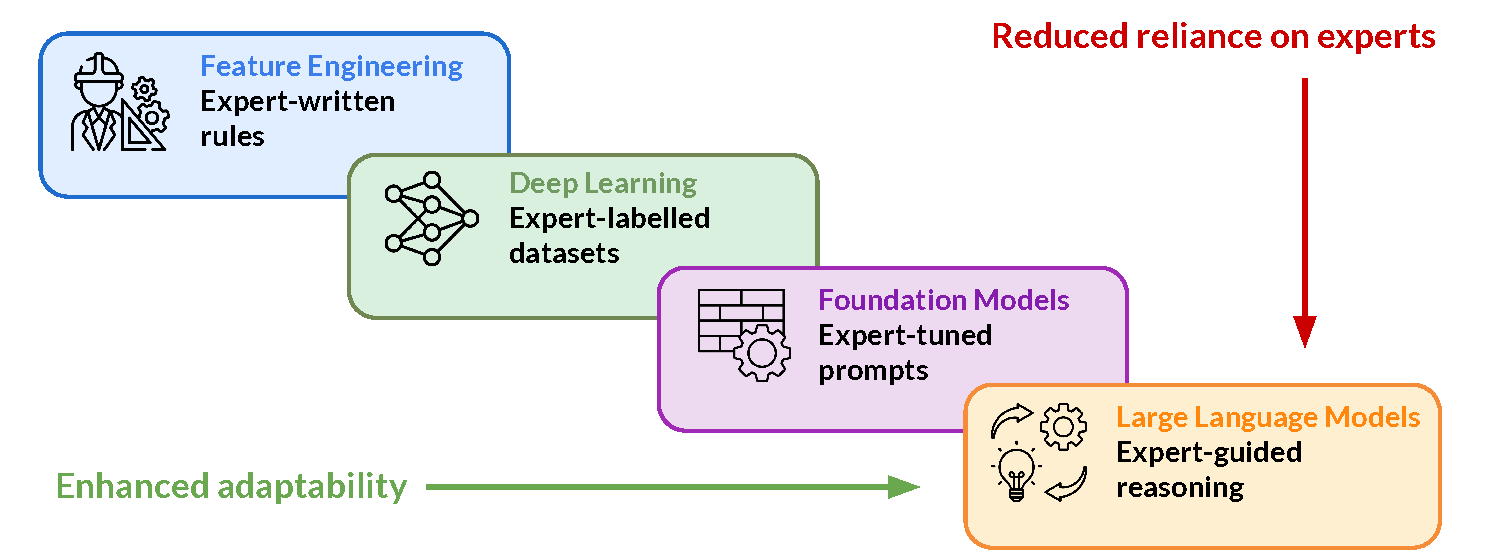
\includegraphics[width=\textwidth]{figs/ai_paradigms.pdf}
\caption{Automated segmentation approaches arranged by their adaptation mechanisms. R4Tun extends the foundation-model pipeline by adding LLM-driven parameter adaptation constrained by expert-guided reasoning.}
\label{fig:paradigms}
\end{figure*}

Three main approaches exist for tunnel point-cloud segmentation (see Fig.~\ref{fig:paradigms} and Section~\ref{sec:related}). Feature-engineering rules are interpretable but brittle under changed conditions~\citep{weidner2024generalized}. Supervised deep-learning models generalise through data but require large labelled datasets and periodic retraining, while lacking auditability~\citep{cha2024deep, su2024review}. Foundation-model pipelines bypass annotation by leveraging models pre-trained on large datasets~\citep{bommasani2021foundation, kirillov2023sam}, but remain sensitive to expert-tuned processing parameters. None of the existing tunnel segmentation approaches reviewed above fully addresses both adaptability to new conditions and the auditability of the adaptation process. Among foundation-model pipelines, SAM4Tun~\citep{ye2025sam4tun} combines point-cloud preprocessing with SAM-based prompting~\citep{kirillov2023sam} and has demonstrated strong performance under expert tuning. However, the pipeline is highly sensitive to its many processing parameters. When tunnel geometry or scanning conditions depart from the tuning reference, performance can degrade, and identifying which parameters require adjustment demands repeated expert intervention.

\hl{Because recent LLMs can perform multi-step reasoning over structured inputs, parameter adaptation can be framed as a diagnostic task in which the model ingests context and proposes bounded adjustments.} LLMs have been applied to engineering workflows including chemical synthesis planning~\citep{bradley2023chemcrow}, multi-agent coordination for complex project tasks~\citep{qian2024chatdev, hong2024metagpt, chen2024comm, ghafarollahi2024protagents}, and manufacturing decision support~\citep{garcia2024manufacturing}. However, these studies do not address parameter adaptation in infrastructure inspection pipelines. We propose R4Tun, an LLM-driven adaptation system that extends the SAM4Tun pipeline by adjusting stage parameters in response to changing tunnel conditions, thereby reducing the need for per-tunnel expert retuning. The framework provides each agent with three context components (memory, state, and knowledge), from which it produces bounded parameter updates via stepwise prompting. \hl{We evaluate whether this context improves segmentation adaptability across regular and complex tunnels, and whether the adaptation behaviour is consistent across independent LLMs.}

This paper makes the following contributions:
\begin{enumerate}
\item A framework design in which LLM agents adapt the parameters of the SAM4Tun pipeline using structured context.
\item \hl{Empirical evidence from cumulative ablation across 30 tunnels suggesting that intermediate pipeline state is an important contributor to adaptation.}
\item \hl{Cross-LLM validation showing that three independent LLMs (Opus-4.6, GPT-5.4, Gemini-3-Flash) exhibit similar adaptation patterns and emphasise a consistent subset of critical parameters.}
\end{enumerate}

The rest of this paper is organised as follows. Section~\ref{sec:related} reviews related work. Section~\ref{sec:methods} presents methodology, including the R4Tun architecture, dataset, experimental design, and evaluation. Section~\ref{sec:results} reports results. Section~\ref{sec:discussion} discusses findings, implications, and limitations. Section~\ref{sec:conclusions} concludes.

% ══════════════════════════════════════════════════════════════════════════
\section{\hl{Related work}}\label{sec:related}
% ══════════════════════════════════════════════════════════════════════════

\subsection{Feature engineering versus deep learning}

Tunnel point-cloud segmentation has advanced through two major generations of methods, each solving one problem while leaving another open (auditability vs. adaptability). Feature-engineering approaches encode domain knowledge into deterministic geometric rules: centreline fitting via RANSAC~\cite{fischler1981ransac}, density-based surface clustering~\cite{ester1996dbscan}, and multi-scale curvature analysis~\cite{pauly2002}. Those methods remain widely used in safety-critical inspection because their logic is explicit and auditable~\cite{weidner2024generalized}. However, each rule embeds assumptions about tunnel geometry and point-cloud characteristics (diameter, ring spacing, joint pattern, point density), and changing any of these requires manual reconfiguration by a domain expert. Supervised deep-learning methods, such as PointNet++~\cite{qi2017pointnet}, RandLA-Net~\cite{hu2020randla}, Mask3D~\cite{schult2023mask3d}, and TD3D~\cite{kolodiazhnyi2024td3d}, learn features directly from annotated point clouds and can generalise across similar conditions present in the training set. \hl{Yet they require large labelled tunnel datasets that remain scarce}~\cite{su2024review}, demand retraining for new tunnel conditions, and provide no mechanism for an engineer to trace or override a segmentation decision~\cite{cha2024deep}.

\hl{Therefore, for inspection operators, deploying to a new tunnel type requires either re-engineering rules, collecting new training data, or accepting degraded performance without a systematic diagnostic mechanism.}

\subsection{Foundation-model pipelines}

To the best of our knowledge, robust direct 3D point-cloud segmentation of infrastructure at tunnel scene scale remains an open challenge for current foundation models. Existing 3D foundation models target common object recognition on curated datasets and do not transfer to large, noisy tunnel point clouds ~\cite{liu2023openshape, guo2023pointbind, xu2024pointllm}. As a result, practical tunnel pipelines often project 3D data into 2D representations to leverage mature vision foundation models pre-trained on large-scale image datasets, thereby bypassing the annotation bottleneck. SAM~\cite{kirillov2023sam} performs class-agnostic segmentation from spatial prompts without task-specific training, and extensions such as SAM2~\cite{ravi2024sam2} for temporal consistency and SEEM~\cite{zou2023segment} for natural-language-guided segmentation are broadening prompt-based segmentation further. These models have been adopted in infrastructure contexts including crack detection~\cite{ravi2024cracksam} and Scan-to-BIM workflows~\cite{wang2024omni}.

For tunnel linings, SAM4Tun~\cite{ye2025sam4tun} combines geometric preprocessing (unfolding, denoising, enhancing) with foundation model 2D segmentation, achieving strong segmentation without training data. However, this pipeline depends on numerous stage-specific parameters that encode assumptions about the reference tunnel's diameter, ring length, point density, and joint patterns. When a new tunnel departs from the reference, these parameters become misspecified and the pipeline degrades silently, without signalling which parameters fail or why. \hl{This sensitivity is not unique to SAM4Tun: any multi-stage pipeline that chains domain-specific preprocessing with a foundation model inherits it. While foundation models have reduced the reliance on labelled data, they have made the pipeline's dependence on hand-tuned parameters more explicit, without alleviating the need for expert parameter tuning.}

\subsection{LLM reasoning}

Recent LLM advances have introduced explicit reasoning capabilities relevant to the parameter-adaptation problem. CoT reasoning~\cite{wei2023cot} enables step-by-step logical traces. Training techniques, especially reinforcement learning~\cite{deepseek2025analysis, openai2025o3, xiang2025metacot}, produce models capable of decomposing complex problems and self-verifying intermediate steps. Multi-agent architectures coordinate specialized roles through shared context~\cite{hong2024metagpt, qian2024chatdev, chen2024comm}, and context engineering influences reasoning quality through the careful design of information provided to models~\cite{xu2024retrieval, mei2025survey}.

\hl{In tunnelling segmentation, however, no prior work has applied LLM-based reasoning to a key challenge in foundation-model pipelines: retuning a parameter-sensitive system to new conditions while preserving the engineer's ability to inspect and override each decision. We therefore introduce an LLM-based reasoning framework that retunes parameter-sensitive pipelines per tunnel using expert-guided context and explicit rationale.}


% ══════════════════════════════════════════════════════════════════════════
\section{Methodology}\label{sec:methods}
% ══════════════════════════════════════════════════════════════════════════

\subsection{Task definition}\label{sec:problem-def}

The task is semantic segmentation of segmental tunnel linings from terrestrial laser scanning (TLS) point clouds. Given a raw point cloud of a tunnel section, the goal is to assign each point a structural label: background, key block~(K), base blocks (B1,~B2), and adjacent blocks (A1--A3), with an additional A4 class for 7-segment complex tunnels. The unit of analysis is a tunnel subset spanning multiple rings selected from the Seg2Tunnel benchmark. 

The practical problem is that the fixed configuration of the open-source SAM4Tun achieves a mean mIoU of 0.291 on regular tunnels, but only 0.042 on complex tunnels whose geometry departs from the tuning reference. As noted above, the pipeline provides no diagnostic feedback when parameters become misspecified.

\subsection{Baseline: SAM4Tun}\label{sec:baseline}

R4Tun complements rather than replaces SAM4Tun~\cite{ye2025sam4tun}. The baseline pipeline architecture is outlined first. SAM4Tun processes tunnel point clouds through four sequential stages:

\textbf{Stage~1-Unfolding} (Fig.~\ref{fig:stage-u}) establishes a cylindrical coordinate system for the tunnel. It slices the point cloud at regular longitudinal intervals, fits an ellipse to each cross-section via RANSAC~\cite{fischler1981ransac}, and selects the model with the highest inlier support. The per-slice ellipse centres are interpolated into a smooth centreline that defines the cylindrical frame~$(r, \theta, h)$. The 3D tunnel surface is then projected into a 2D panoramic image in which each pixel encodes the radial distance to the centreline, producing a stable depth representation for downstream filtering and segmentation.

\begin{figure*}[t]
\centering
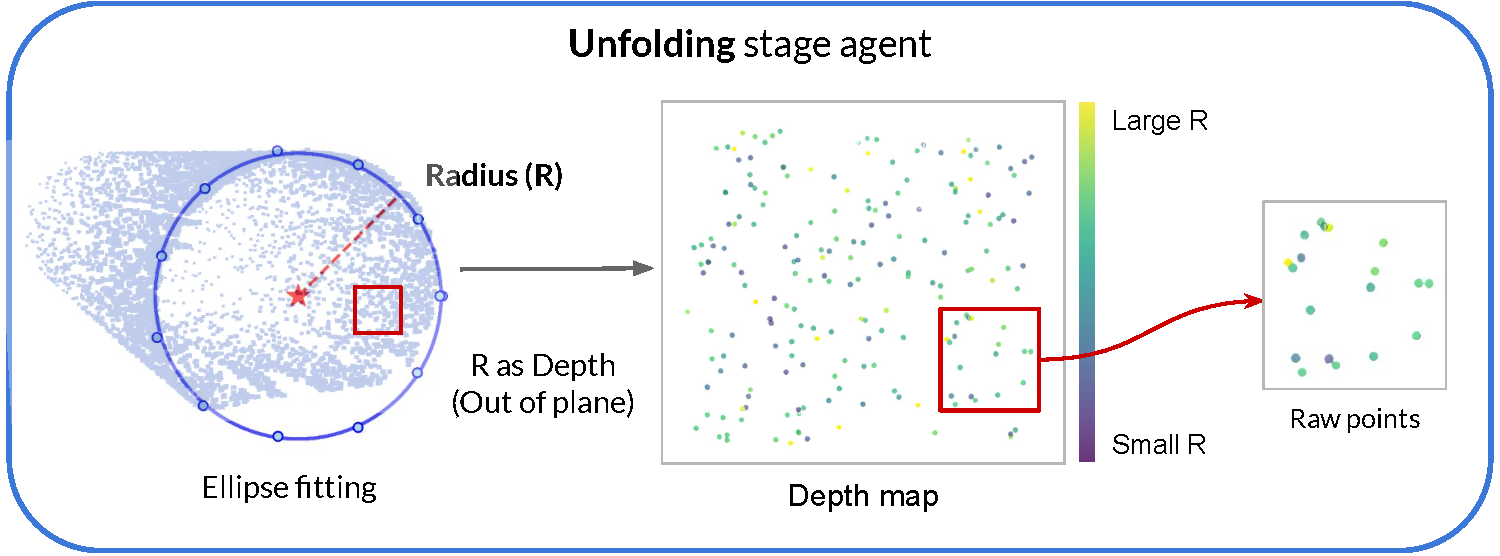
\includegraphics[width=0.8\textwidth]{figs/stage_u.pdf}
\caption{Stage 1-Unfolding. Left: fitted tunnel cross-section used to determine the reference centre and radius for cylindrical unfolding. Centre: 2D panoramic depth map derived from the 3D point cloud. Right: zoomed region of the unfolded map showing radial-distance encoding.}
\label{fig:stage-u}
\end{figure*}

\textbf{Stage~2-Denoising} (Fig.~\ref{fig:stage-d}) removes non-structural artefacts (rails, cables, and scattered points) that would otherwise interfere with segmentation. The algorithm applies grid-based radial-density filtering inspired by the DBSCAN clustering principle~\cite{ester1996dbscan}, grouping points by local density in cylindrical coordinates. Dense, connected regions are retained as tunnel surfaces while isolated points are rejected as noise. A pair of radial masks~($R_\mathrm{low}$, $R_\mathrm{high}$) constrains filtering to the expected tunnel radius, preserving joint boundaries and ring edges while discarding outliers beyond the lining surface. The result is a clean, continuous surface representation suitable for curvature analysis and interpolation in the next stage. 

\begin{figure*}[t]
\centering
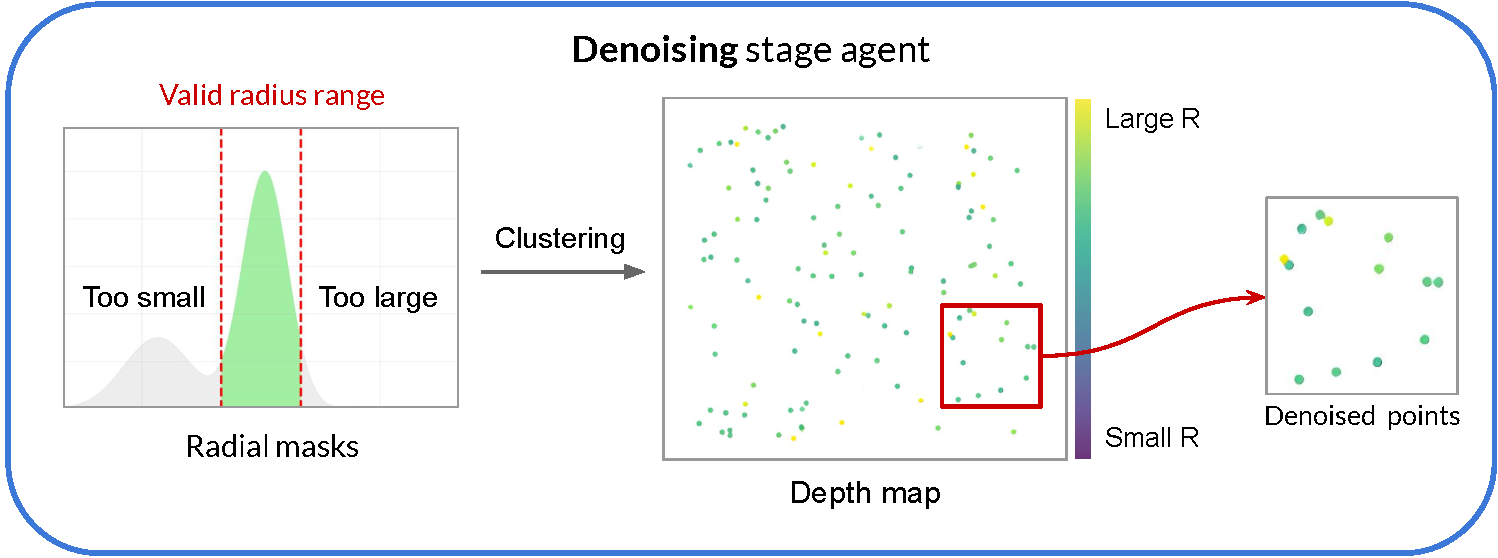
\includegraphics[width=0.8\textwidth]{figs/stage_d.pdf}
\caption{Stage 2-Denoising. Left: radial-distance distribution used to filter points outside the expected tunnel lining surface. Centre: unfolded 2D depth map after filtering, showing the cleaned point distribution. Right: zoomed region of the denoised map.}
\label{fig:stage-d}
\end{figure*}

\textbf{Stage~3-Enhancing} (Fig.~\ref{fig:stage-e}) improves geometric continuity and surface completeness before projection into the 2D depth map. Local curvature is estimated on neighbourhood points to guide point insertion: new points are placed between neighbours whose curvature difference is small (smooth panel regions), while high-curvature areas (joint boundaries and ring edges) are preserved intact. A three-stage progressive upsampling scheme inserts additional points at progressively finer resolutions to maintain surface continuity without blurring structural boundaries. Pixel-level interpolation then refines outlier points at joint locations. The enhanced surface is projected into a panoramic depth map that balances smooth panel regions with sharply defined joint boundaries. 

\begin{figure*}[t]
\centering
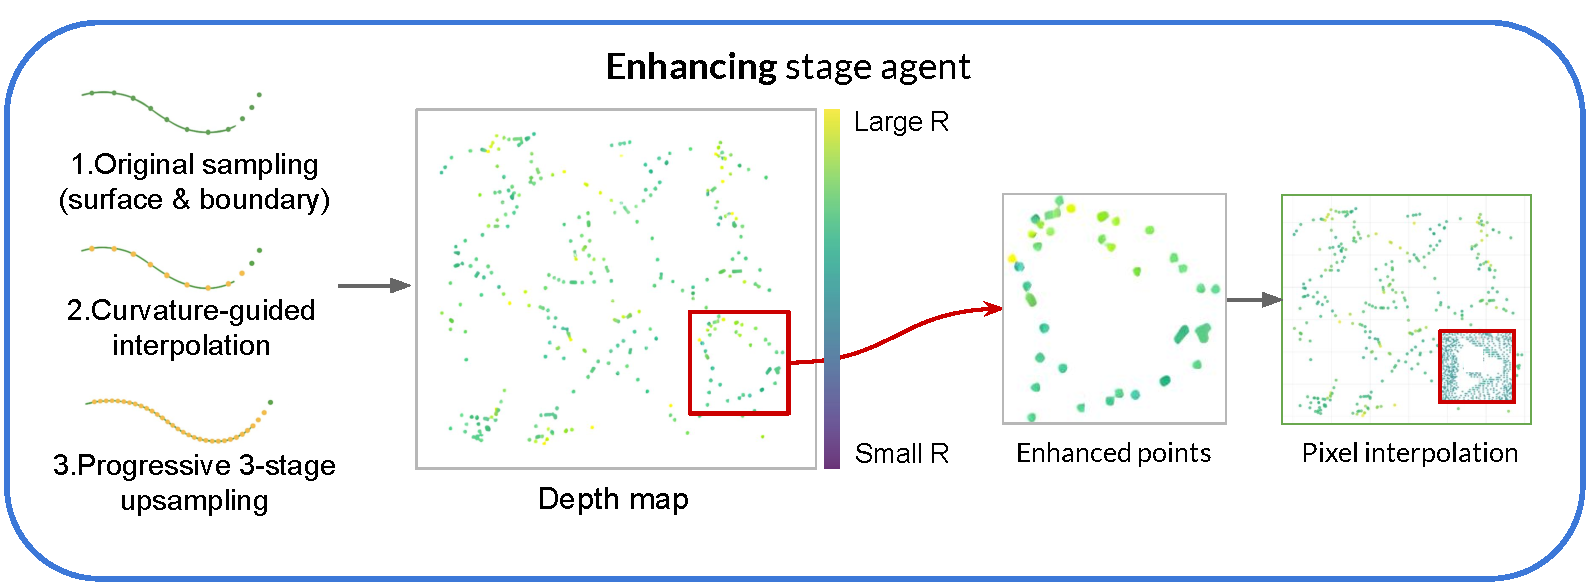
\includegraphics[width=0.8\textwidth]{figs/stage_e.pdf}
\caption{Stage 3-Enhancing. Left: curvature-guided surface and boundary interpolation along the tunnel lining, showing original sampling, curvature-guided insertion, and progressive three-stage upsampling. Centre: unfolded 2D depth map after enhancement, where inserted points improve geometric continuity; the red box highlights a local region of interest. Right: zoomed views of the highlighted region, showing added points and pixel-level interpolation.}
\label{fig:stage-e}
\end{figure*}

\textbf{Stage~4-Segmenting} (Fig.~\ref{fig:stage-p}) combines boundary detection and SAM segmentation into a single workflow. First, a Hough-transform-based detector~\cite{duan2023high} extracts linear features from the enhanced depth map that correspond to ring joint boundaries. Detected lines are filtered by orientation (oblique, horizontal, vertical) with separate Hough thresholds and merged when closer than a distance tolerance. The confirmed boundaries are then used to construct template-based prompts for key, base, and adjacent segments, which are passed to SAM~\cite{kirillov2023sam}. SAM produces 2D segment masks on the panoramic image, which are reprojected into 3D point labels via the stored pixel-to-point mapping from Stage~1. 

\begin{figure*}[t]
\centering
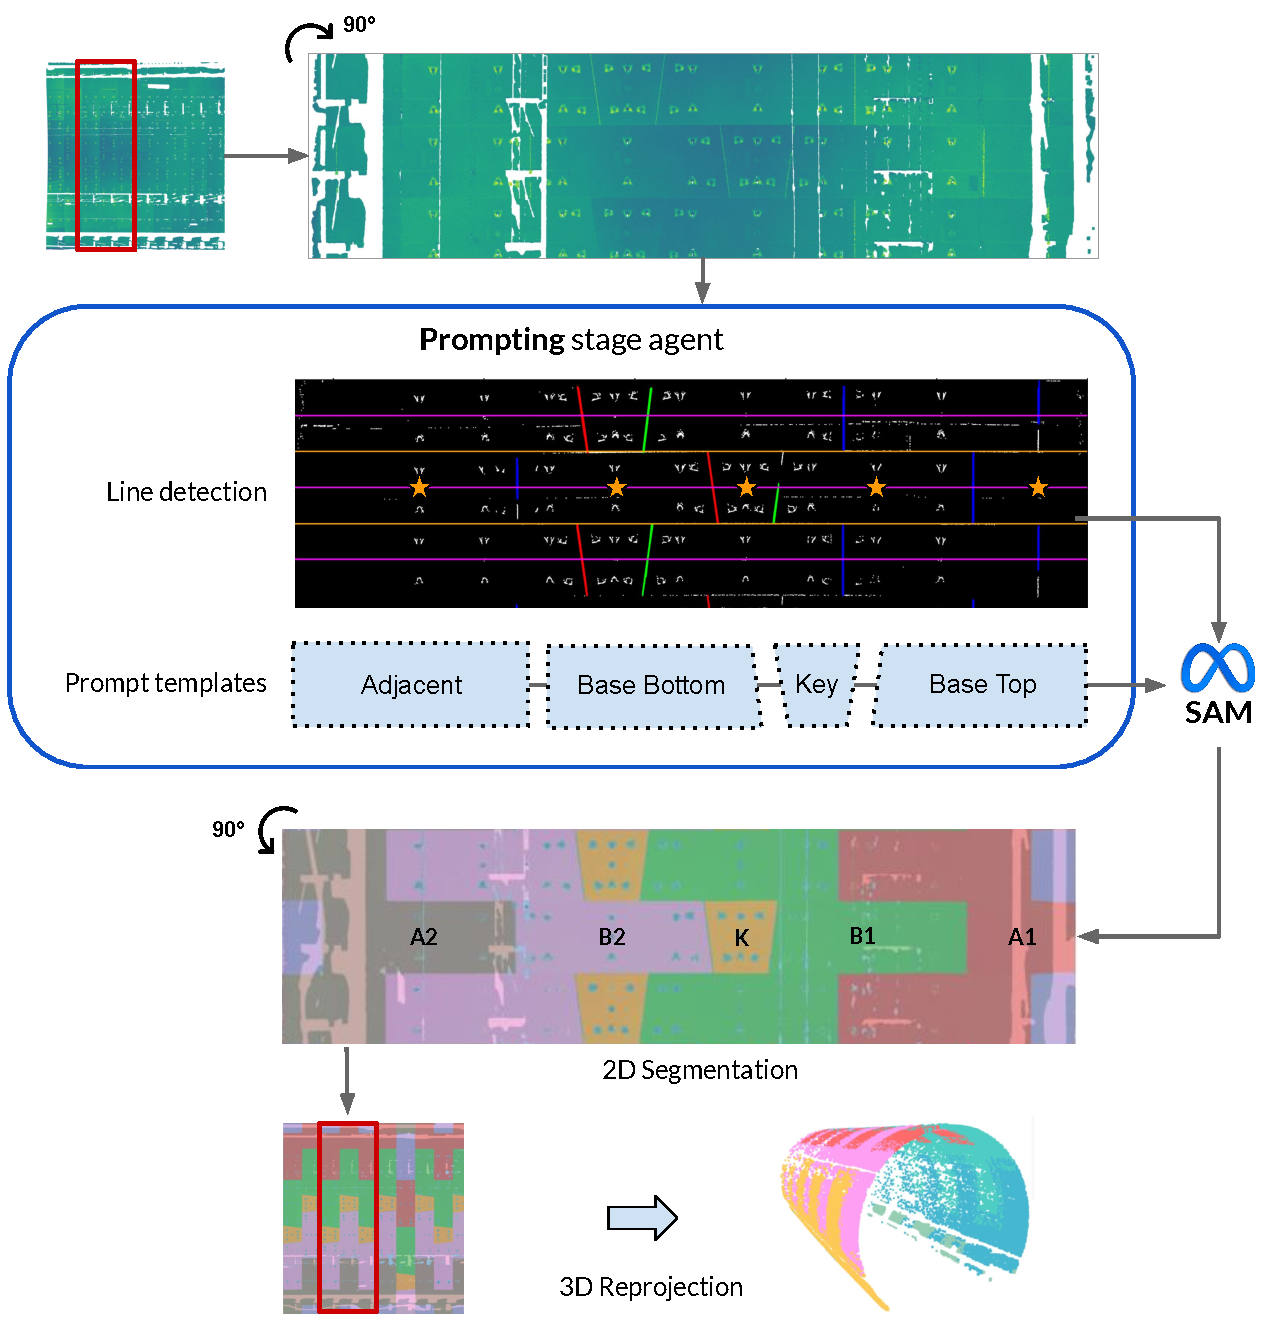
\includegraphics[width=0.8\textwidth]{figs/stage_p.pdf}
\caption{Stage~4-Segmenting: Hough-transform line detection to identify ring boundaries, constructs template-based prompts, and feeds them to SAM~\cite{kirillov2023sam}, which produces 2D segment masks that are reprojected into 3D. (Note: rotation is shown for visualisation purposes only.)}
\label{fig:stage-p}
\end{figure*}

The pipeline contains approximately 80 tuneable processing parameters. All parameters were expert-tuned on a reference tunnel (diameter 5.60\,m, density 2{,}466\,pts/m$^3$, mIoU\,=\,0.531); full parameter tables are provided in Appendix~\ref{app:params}. In this study, the underlying pipeline stages remain fixed across all conditions; only the parameter values change. The \texttt{sam4tun} baseline applies this single expert-tuned configuration uniformly to all 30 tunnels without per-tunnel adaptation, serving as the fixed-parameter reference against which all adaptive conditions are measured.

\subsubsection{On-site rules baseline}\label{sec:rules-baseline}

To isolate the contribution of LLM reasoning from simple family-level parameter adjustment, a deterministic rules baseline is included. This baseline represents what a practitioner could achieve using only \emph{field-observable} inputs available before running the pipeline: the nominal tunnel diameter (from design drawings or tape measurement), ring length, segment count per ring, and tunnel family. No characteriser output, pipeline intermediate state, or domain-knowledge document is used.

The rules adjust five parameters from the sam4tun defaults: (1)~\texttt{diameter} in unfolding is set to the measured value; (2)~the denoising radial masks (\texttt{mask\_r\_low}, \texttt{mask\_r\_high}) and fallback cutoff are derived from diameter$/2 \pm 0.15$\,m; (3)~\texttt{ring\_spacing\_constant} in detection is set to the ring length; and (4)~\texttt{segment\_per\_ring} and the SAM template geometry are set to match the tunnel family (6-segment for T1--T3, 7-segment for T4--T5). All other parameters retain their sam4tun values. The complete rule specification is provided in Appendix~\ref{app:rules}.

\subsection{R4Tun}\label{sec:method}

R4Tun supplements the SAM4Tun pipeline with an LLM-driven adaptation layer that adjusts parameters per tunnel without modifying the underlying algorithms (Fig.~\ref{fig:architecture}). Given a new tunnel point cloud, a characteriser first extracts raw geometric properties (diameter, density, coordinate ranges; full field list in Appendix~\ref{app:chars}). Each of the four stages (unfolding, denoising, enhancing, and segmenting) has a dedicated LLM agent that adapts its parameters. In the segmenting stage, the adapted prompts are passed to SAM, and the resulting 2D masks are reprojected onto the 3D point cloud without further LLM intervention.

For each agent-driven stage, (i)~the orchestrator assembles a prompt from the current context level (Section~\ref{sec:context-comp}); (ii)~the LLM reasons over this prompt via CoT and returns an adapted parameter JSON (Section~\ref{sec:cot}); (iii)~the stage runs with the adapted parameters; and (iv)~a characteriser plugin extracts statistics from the output, updating the state available to subsequent stages. Each stage’s parameters are adapted from the expert-tuned reference configuration together with the cumulative state produced by earlier stages. The stage scripts and evaluation code are identical across all ablation conditions; only the parameter JSONs change. A worked example of this process is provided in Appendix~\ref{app:cot}. After the final segmentation, per-point labels are evaluated against ground truth using mean Intersection over Union (mIoU) as the primary metric.

\begin{figure*}[t]
\centering
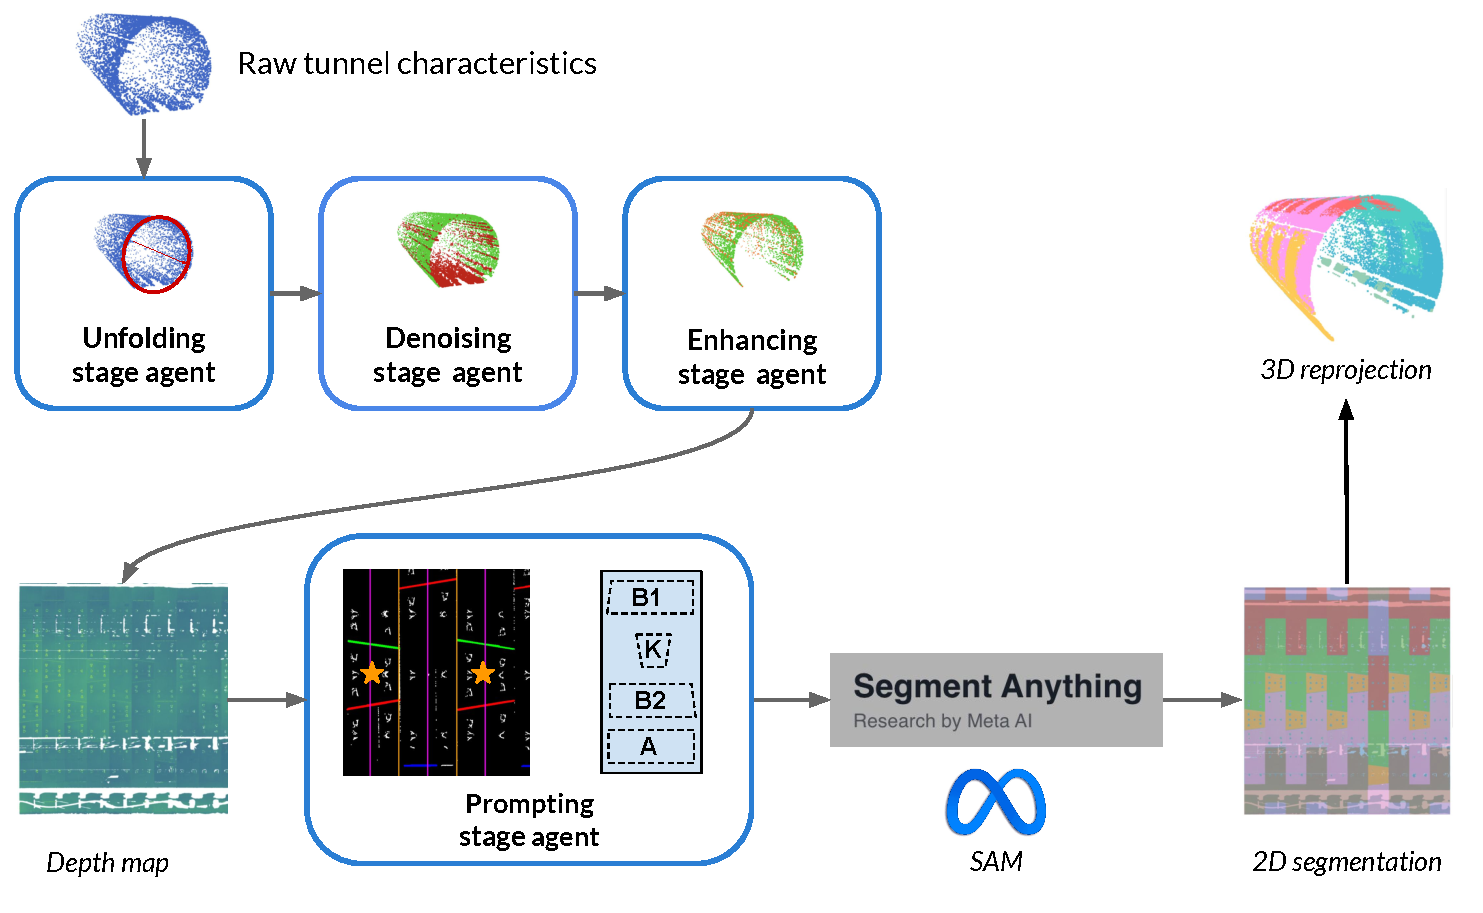
\includegraphics[width=0.8\textwidth]{figs/r4tun_pipeline.pdf}
\caption{The R4Tun multi-agent architecture for tunnel segmentation. Four stage agents (unfolding, denoising, enhancing, and segmenting) adapt their parameters through LLM reasoning to generate segmentation.}
\label{fig:architecture}
\end{figure*}

\begin{figure*}[t]
\centering
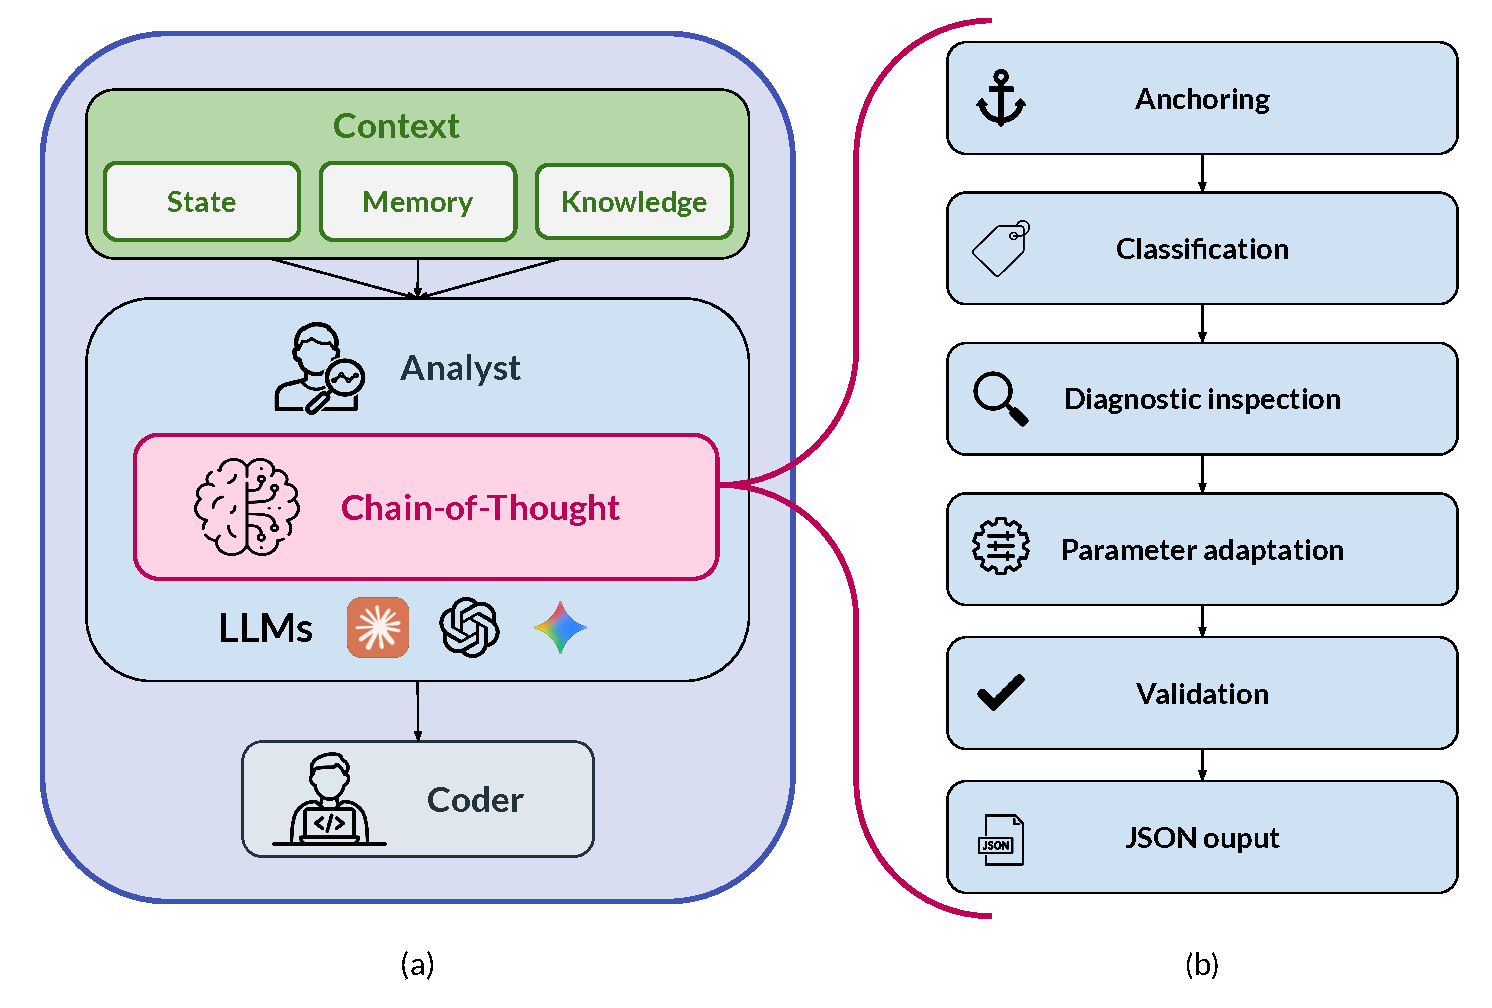
\includegraphics[width=0.8\textwidth]{figs/agent_design.pdf}
\caption{The left column (a) shows R4Tun stage agent architecture. Each agent maintains an evolving context that informs an LLM analyst component performing CoT reasoning. The right column (b) shows the five CoT phases: (1) Referencing, (2) Diagnostic inspection, (3) Parameter adaptation, (4) Validation, and (5) JSON output.}
\label{fig:agent-design}
\end{figure*}

\subsubsection{Agent design}\label{sec:agent-design}

Each of the four stage agents is a self-contained unit comprising two components: a \emph{context} (Section~\ref{sec:context-comp}) (Fig.~\ref{fig:agent-design}a), and an \emph{LLM analyst} function that constructs the full LLM prompt and parses the returned JSON. Within this prompt, the analyst embeds a five-step CoT protocol (Section~\ref{sec:cot}) (Fig.~\ref{fig:agent-design}b) that guides the LLM through referencing, diagnostic inspection, parameter adaptation, validation, and JSON output. The LLM then outputs a single schema-conformant parameter JSON, which the corresponding pipeline stage executes unchanged. Because every parameter change is logged alongside a generated textual rationale, engineers can review and, where necessary, override adaptation decisions.

\subsubsection{Context design}\label{sec:context-comp}

Each stage agent receives structured context comprising three components: memory, state and knowledge (Fig.~\ref{fig:agent-design}a).

\textbf{Memory} stores the reference tunnel's characteristics (a JSON file containing geometry, point density, coordinate ranges, nearest-neighbour distances) alongside the expert-tuned reference parameters. The agent compares the current tunnel's characteristics against this reference to quantify deviation and adjust its parameters. Memory is static: it does not change between stages.

\textbf{State} captures cumulative geometric and statistical properties after each pipeline stage executes. These JSON summaries are injected into subsequent agents' prompts, and the state grows as stages execute. Importantly, state alone does not prescribe parameter changes: the numeric summaries must be interpreted in the context of parameter semantics and tunnel conditions before they can inform parameter updates.

\textbf{Knowledge} supplies domain-specific guidance in human-readable markdown documents. Each stage has its own knowledge document covering: tunnel-type taxonomy; parameter semantics and empirically validated ranges; and diagnostic rules linking characteristics to parameter adjustments. Knowledge is authored once and shared across all tunnels.

\subsubsection{CoT design}\label{sec:cot}

CoT reasoning provides the analytical structure for each agent's decision-making (Fig.~\ref{fig:agent-design}b). Each stage agent follows a five-step protocol: (i)~\emph{referencing} compares the current tunnel's characteristics against the stored reference to quantify deviation; (ii)~\emph{diagnostic inspection} attributes the deviation to a plausible cause and identifies which stage parameters are implicated; (iii)~\emph{parameter adaptation} proposes bounded updates within empirically predefined ranges, grounded in the diagnostic evidence and domain knowledge; (iv)~\emph{validation} performs a lightweight consistency check to confirm that the proposed values satisfy logical constraints; and (v)~\emph{JSON output} packages the selected parameters and their reasoning trace into a single schema-conformant JSON object, which is executed by the underlying pipeline-stage function. A worked example of the full five-step trace is provided in Appendix~\ref{app:cot}.

\subsection{Experimental setup}\label{sec:exp-setup}

\subsubsection{Dataset}\label{sec:dataset}

We selected 30 tunnel subsets from the Seg2Tunnel benchmark (Table~\ref{tab:dataset}). These subsets span the main axes of variation in segmental tunnel geometry (diameter, ring length, segment count, key-block layout, and point-density distribution), providing a controlled basis for evaluating adaptation across tunnel families.

Staggered and continuous tunnels are grouped as ``regular'' ($n = 13$): they share the 5.5\,m nominal diameter, 1.2\,m ring spacing, six segments per ring, and, most importantly, regular patterns of key-block positions similar to the reference. Complex tunnels ($n = 17$) depart from that reference in multiple coupled ways: inner diameter increases by 36\% (7.5\,m), ring length by 50\% (1.8\,m), and each ring adds a seventh segment with a complex interleaved key-block arrangement. In addition, off-axis scanning yields non-uniform sampling, partial circumferential coverage, and angle-dependent range and incidence. Together, these differences alter both the geometry visible in the point cloud and the semantic targets the pipeline must recover. Consequently, a fixed parameter set cannot be assumed to transfer from the regular reference; these conditions constitute the primary stress test for whether R4Tun can adapt the same algorithmic pipeline to off-design tunnel conditions. Ground-truth labels are per-point structural class annotations provided by the Seg2Tunnel benchmark; they are used for evaluation only and are not provided to the LLM or pipeline during adaptation.

\begin{table*}[t]
\caption{Dataset properties.}\label{tab:dataset}
\begin{tabular*}{\textwidth}{@{\extracolsep{\fill}} l l l l @{}}
\toprule
 & \multicolumn{2}{c}{Regular (T1, T2, T3)} & Complex (T4, T5) \\
\cmidrule(lr){2-3}\cmidrule(l){4-4}
Property & Staggered (T1, T2) & Continuous (T3) & \\
\midrule
Inner diameter & 5.5\,m & 5.5\,m & 7.5\,m \\
Ring length & 1.2\,m & 1.2\,m & 1.8\,m \\
Segments/ring & 6 & 6 & 7 \\
Joint type & Staggered & Continuous & Complex interleaved \\
Key-block position & \parbox[t]{0.30\textwidth}{\raggedright A ring-to-ring repeating pattern} & \parbox[t]{0.20\textwidth}{\raggedright A fixed ring-wise order} & \parbox[t]{0.20\textwidth}{\raggedright No repeating pattern} \\
Scanning & Single-station & Multi-station & Single-station, offset \\
Eval.\ schema & 6-class & 6-class & 7-class \\
Count & 10 subsets & 3 subsets & 17 subsets \\
\bottomrule
\end{tabular*}
\end{table*}

\subsubsection{Experimental design}\label{sec:comparators}

The experiment follows a cumulative ablation design with five conditions (Table~\ref{tab:ablation}). The on-site rules baseline (Section~\ref{sec:rules-baseline}) uses only field-observable inputs and no LLM. Levels~1--3 progressively provide the LLM with richer context, enabling the cumulative ablation to attribute improvements to specific components.

\begin{table}[ht]
\caption{Ablation conditions.}\label{tab:ablation}
\begin{tabular*}{\tblwidth}{@{} c l l >{\raggedright\arraybackslash}p{2.75cm} @{\hspace{0.7em}}@{}}
\toprule
Level & Code & Condition & Context \\
\midrule
0 & SAM4Tun & Baseline & Fixed default parameters \\
--- & Rules & On-site rules & Field-observable inputs (diameter, family, ring length) \\
1 & m & Memory & Reference characteristics + parameters \\
2 & m+s & Memory+State & + intermediate pipeline outputs \\
3 & m+s+k & \begin{tabular}[t]{@{}l@{}}Memory + State + \\ Knowledge\end{tabular} & + domain knowledge \\
\bottomrule
\end{tabular*}
\end{table}

Level~0 (\texttt{SAM4Tun}) is the fixed expert-tuned baseline with no LLM involvement. The rules condition represents a practitioner applying family-level adjustments from drawings alone, without LLM assistance. Levels~1--3 progressively provide the LLM with richer context. To assess whether adaptation behaviour depends on a specific LLM, each LLM condition was run with three independent LLMs (Opus-4.6, GPT-5.4, and Gemini-3-Flash) under identical prompts. Across models, the pipeline code, evaluation scripts, and prompt structure were held constant, while the context content varied by ablation level. Because vendor-specific API defaults (e.g., temperature settings; Table~\ref{tab:llm-config}) were not fully harmonised, the cross-model comparison should be interpreted primarily as a robustness check rather than a perfectly controlled benchmark. Each of the three ablation conditions was run once per LLM for all 30 tunnels, yielding $3 \times 3 \times 30 = 270$ pipeline executions plus 30 baseline runs and 30 rules runs. All three LLMs were accessed via their respective commercial APIs (Table~\ref{tab:llm-config}). No model-specific prompt tuning was performed.

\begin{table}[ht]
\caption{LLM configuration.}\label{tab:llm-config}
\begin{tabular*}{\tblwidth}{@{} l l @{}}
\toprule
Setting & Value \\
\midrule
Models & Opus-4.6, GPT-5.4, Gemini-3-Flash \\
Max tokens & 16{,}384 \\
Temperature & Default \\
Timeout & 300\,s per call \\
Prompt format & Markdown with JSON code \\
Failure handling & JSON extraction fail $\rightarrow$ log \& error \\
\bottomrule
\end{tabular*}
\end{table}



Pipeline execution used a single NVIDIA RTX~5060 GPU. Adapted parameter files and CoT reasoning traces were logged for all runs, enabling post-hoc sensitivity analysis (Section~\ref{sec:sensitivity-method}).

\subsubsection{Evaluation metrics}\label{sec:metrics}

Segmentation quality is measured by mean Intersection-over-Union (mIoU):
\begin{equation}
\text{IoU}_c = \frac{\text{TP}_c}{\text{TP}_c + \text{FP}_c + \text{FN}_c}, \qquad
\text{mIoU} = \frac{1}{C} \sum_{c=1}^{C} \text{IoU}_c,
\end{equation}
where $C = 6$ (regular) or $C = 7$ (complex). mIoU is the primary metric. Per-class IoU is reported to assess whether improvements are broad or concentrated in specific structural classes.

For each condition and LLM, we computed paired per-tunnel improvements as $\Delta_i = \mathrm{mIoU}_{\text{condition},i} - \mathrm{mIoU}_{\text{baseline},i}$, with $n=13$ for regular tunnels, $n=17$ for complex tunnels, and $n=30$ overall. We summarise these paired improvements using three standard statistics: (i) two-sided paired $t$-test $p$-values ($\alpha = 0.05$) for statistical significance, (ii) paired Cohen's $d$ for effect size, and (iii) bootstrap 95\% confidence intervals (CIs) for the mean improvement.

\subsubsection{Sensitivity analysis}\label{sec:sensitivity-method}

To assess the robustness of adapted parameters, we analysed 270 adapted parameter runs ($30~\text{tunnels} \times 3~\text{LLMs} \times 3~\text{conditions} $). For each parameter, we report the \emph{coefficient of variation}~(CV):
\begin{equation}\label{eq:cv}
\text{CV} = \frac{s}{\lvert\bar{v}\rvert},
\end{equation}
where $\bar{v} = \frac{1}{N}\sum_{i=1}^{N} v_i$ and $s = \sqrt{\frac{1}{N-1}\sum_{i=1}^{N}(v_i - \bar{v})^2}$ are the mean and standard deviation of the adapted values $\{v_i\}_{i=1}^{N}$ across $N = 30$~tunnels. CV measures how much a parameter changes from tunnel to tunnel: (i)~a high CV ($\geq 0.06$) identifies parameters that are \emph{tunnel-responsive}; (ii)~$\text{CV} \approx 0$ indicates \emph{baseline corrections} that take the same improved value on every tunnel regardless of geometry. We further examine \emph{cross-LLM consistency}: for parameters that always trigger adaptation, we compare the adapted values, tunnel counts, and tunnel-family clustering produced by each LLM independently.






% ══════════════════════════════════════════════════════════════════════════
\section{Results}\label{sec:results}
% ══════════════════════════════════════════════════════════════════════════

\subsection{Overall performance}\label{sec:main-results}

Table~\ref{tab:main-results} summarises mean mIoU across conditions and LLMs. Under the full memory+state+knowledge (m+s+k) design, overall mIoU rises from 0.150 (baseline) to 0.313--0.328 across the three LLMs ($p < 0.0001$, paired Cohen's $d = 1.44$--$1.94$). The improvement holds across both tunnel families (Fig.~\ref{fig:ablation-bar}). Regular tunnels improve from 0.291 to 0.495--0.535 (effect sizes $d = 1.4$--$2.2$). Complex tunnels---where the baseline drops to mIoU\,=\,0.042 because several pipeline assumptions no longer match the tunnel conditions---improve to 0.169--0.177 ($d = 1.2$--$2.4$), an absolute increase of 0.127--0.135 mIoU. Per-class IoU analysis (Appendix~\ref{app:perclass}) supports broad improvement across structural classes for regular tunnels and progressive recovery from near-zero baselines for complex tunnels.

\begin{table*}[t]
\caption{Overall segmentation results ($n=30$): mean mIoU and paired $\Delta$mIoU vs baseline with $p$-values, effect sizes, and bootstrap 95\% CIs.}\label{tab:main-results}
\begin{tabular*}{\textwidth}{@{\extracolsep{\fill}} l l c c c @{}}
\toprule
Condition & Statistic & Opus-4.6 & GPT-5.4 & Gemini-3-Flash \\
\midrule
Baseline (sam4tun) & Mean mIoU & 0.150 & 0.150 & 0.150 \\
\midrule
\multirow{5}{*}{Rules ($n=30$)}
  & Mean mIoU & \multicolumn{3}{c}{0.201} \\
  & Mean $\Delta$ & \multicolumn{3}{c}{$+0.051$} \\
  & $p$-value & \multicolumn{3}{c}{0.004} \\
  & Cohen's $d$ & \multicolumn{3}{c}{0.58} \\
  & 95\% CI & \multicolumn{3}{c}{$[0.019,\; 0.083]$} \\
\midrule
\multirow{5}{*}{m}
  & Mean mIoU & 0.144 & 0.182 & 0.199 \\
  & Mean $\Delta$ & $-0.006$ & $+0.032$ & $+0.049$ \\
  & $p$-value & 0.558 & 0.028 & 0.056 \\
  & Cohen's $d$ & $-0.11$ & 0.42 & 0.36 \\
  & 95\% CI & $[-0.027,\; 0.014]$ & $[0.005,\; 0.058]$ & $[0.006,\; 0.101]$ \\
\midrule
\multirow{5}{*}{m+s}
  & Mean mIoU & 0.312 & 0.299 & 0.302 \\
  & Mean $\Delta$ & $+0.162$ & $+0.149$ & $+0.152$ \\
  & $p$-value & $<0.0001$ & $<0.0001$ & $<0.0001$ \\
  & Cohen's $d$ & 1.61 & 1.32 & 1.46 \\
  & 95\% CI & $[0.126,\; 0.198]$ & $[0.110,\; 0.190]$ & $[0.117,\; 0.189]$ \\
\midrule
\multirow{5}{*}{m+s+k}
  & \textbf{Mean mIoU} & \textbf{0.328} & \textbf{0.321} & \textbf{0.313} \\
  & Mean $\Delta$ & $+0.178$ & $+0.171$ & $+0.163$ \\
  & $p$-value & $<0.0001$ & $<0.0001$ & $<0.0001$ \\
  & Cohen's $d$ & 1.61 & 1.94 & 1.44 \\
  & 95\% CI & $[0.139,\; 0.216]$ & $[0.140,\; 0.203]$ & $[0.122,\; 0.203]$ \\
\bottomrule
\end{tabular*}
\end{table*}



\begin{figure*}[t]
\centering
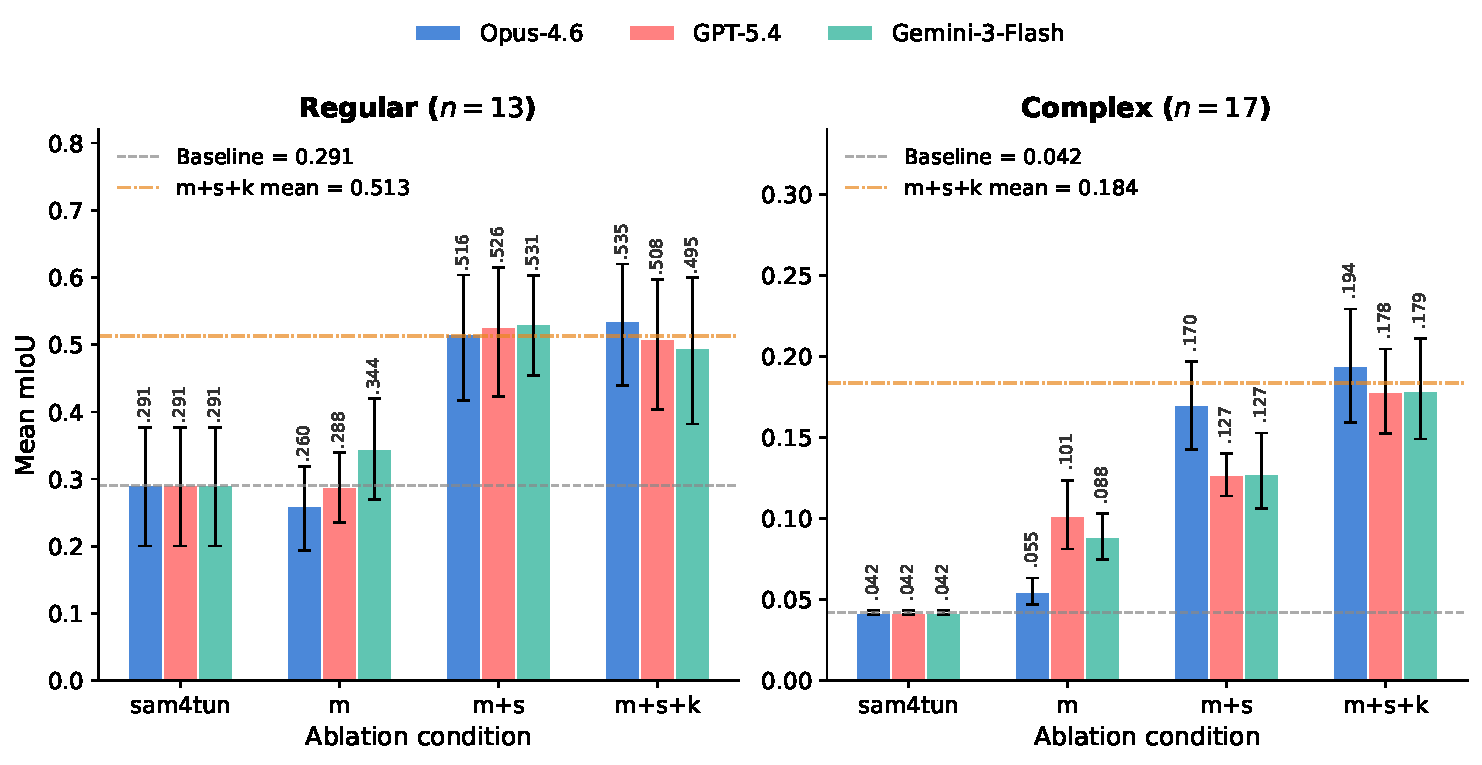
\includegraphics[width=\textwidth]{figs/ablation_bar.pdf}
\caption{Step-wise ablation results split by tunnel family and LLM. State produces the dominant jump for regular tunnels. Error bars represent bootstrap 95\% CIs.}
\label{fig:ablation-bar}
\end{figure*}

\begin{figure}[t]
\centering
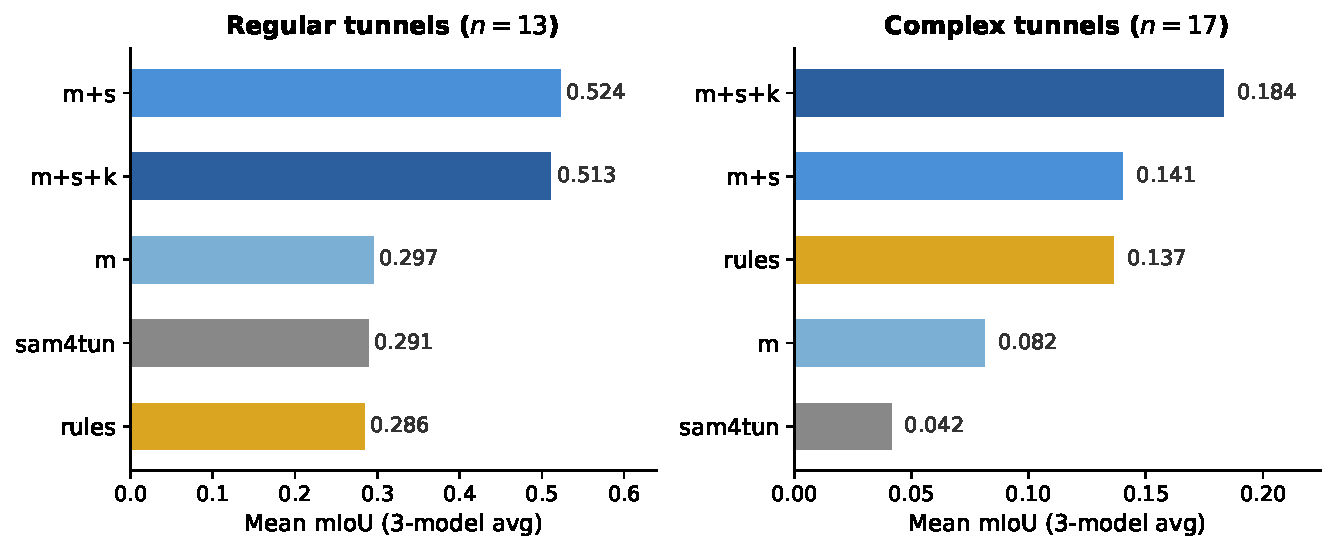
\includegraphics[width=\columnwidth]{figs/rules_comparison.pdf}
\caption{Three-model-average mIoU by condition, sorted by value within each panel. The rules baseline (gold) uses only field-observable inputs; LLM conditions use 3-model means. Three failed rules tunnels are counted as zero.}
\label{fig:rules-comparison}
\end{figure}

\subsection{Ablation analysis}\label{sec:ablation}

To isolate each context component's contribution, Table~\ref{tab:cumulative_miou} reports cumulative mIoU gains at each ablation step. Fig.~\ref{fig:ablation-bar} visualises the step-wise progression for regular and complex families across all three LLMs, and Fig.~\ref{fig:rules-comparison} ranks all five conditions (including the deterministic rules baseline) by their 3-model-average mIoU.

\begin{table}[ht]
\caption{Cumulative mIoU contribution (mean $\Delta$ vs. previous level).}\label{tab:cumulative_miou}
\begin{tabular*}{\tblwidth}{@{} l c c c @{}}
\toprule
Transition & Opus-4.6 & GPT-5.4 & Gemini-3-Flash \\
\midrule
Baseline $\rightarrow$ Rules & \multicolumn{3}{c}{$+0.051$ ($n=30$; 3 failures\,$=$\,0)} \\
Baseline $\rightarrow$ m & $-0.006$ & $+0.032$ & $+0.049$ \\
m $\rightarrow$ m+s & $+0.168$ & $+0.117$ & $+0.103$ \\
\textbf{m+s $\rightarrow$ m+s+k} & $\mathbf{+0.016}$ & $\mathbf{+0.022}$ & $\mathbf{+0.011}$ \\
\bottomrule
\end{tabular*}
\end{table}

\textbf{The on-site rules baseline} achieves mean mIoU\,=\,0.201 ($n=30$; 3 complex tunnels failed due to detection row-count mismatch under default Hough thresholds and are counted as mIoU\,=\,0). On regular tunnels, rules provide negligible improvement over sam4tun ($\Delta = -0.005$, $p = 0.79$), because the sam4tun defaults were already tuned for the 5.5\,m family. On complex tunnels, rules improve substantially ($\Delta = +0.095$, $p = 0.0001$, $d = 1.23$) by correcting the gross diameter and family mismatch, but 3 of 17 tunnels fail outright. Fig.~\ref{fig:rules-comparison} ranks all five conditions by their 3-model-average mIoU: on complex tunnels, rules (0.137) sit between m (0.081) and m+s+k (0.173), while on regular tunnels rules (0.286) trail all LLM conditions beyond memory alone. The LLM conditions produce their largest gains on regular tunnels (mean mIoU 0.495--0.535 vs rules 0.286), where characteriser-state-driven parameters (Hough thresholds, denoising masks tuned to $p_{10}$/$p_{99}$, upsampling targets) provide the additional lift.

\textbf{Memory alone} provides an initial reference but is insufficient, and in some settings it degrades performance. On regular tunnels, especially the staggered subsets, memory alone degrades mIoU by $-0.035$ to $-0.055$. Without intermediate feedback, the agent attempts to adapt parameters but cannot verify whether adjustments improve or degrade the pipeline outputs.

\textbf{State is associated with the largest cumulative improvement.} The m+s condition yields the strongest gain relative to baseline across all three LLMs (all $p < 0.0001$; paired Cohen's $d = 1.32$--$1.61$), and because the memory-only condition is small or inconsistent, most of this cumulative gain appears to be attributable to state. State provides the agent with explicit quantitative evidence of how each stage has transformed the data---radial percentiles for mask bounds, retention rates for denoising aggressiveness, coverage uniformity for upsampling targets. Without state, the agent has only pre-pipeline statistics that may not reflect conditions after unfolding, denoising, or enhancing.

The gain associated with state likely depends on a model's ability to interpret raw numeric summaries (percentiles, counts, ratios) in the context of parameter semantics and map them to appropriate parameter values. We did not test alternative mapping strategies (e.g., regression models or heuristic rules); however, the continuous, multidimensional nature of the characteristic space and the non-trivial parameter interactions suggest that capturing this mapping through static rules alone would require substantial manual engineering effort per tunnel family.

\textbf{Knowledge appears to provide targeted improvements in a subset of tunnels.} Knowledge provides a mean increment of $+0.011$ to $+0.022$ (Cohen's $d = 0.11$--$0.31$, ``small''). Bootstrap CIs on the mean increment straddle zero for all three LLMs. However, 21/30 tunnels show positive increments for Opus~4.6 and GPT-5.4 (one-sided binomial $p = 0.021$), and on complex tunnels 15/17 are positive for GPT ($p = 0.001$). Knowledge is most valuable where it supplies tunnel-family-specific configuration that neither memory nor state can provide (e.g., \texttt{ring\_spacing\_constant}\,=\,1.8 vs 1.2, 7~segments per ring, 7.5/5.5 scaling).

\subsection{Cross-model consistency}\label{sec:consistency}

To assess whether the adaptation is model-dependent or driven by objective tunnel conditions, Table~\ref{tab:cross-model} compares the three LLMs on the full m+s+k condition. All three 95\% CIs overlap, suggesting that the improvement is consistent across the tested LLMs and is not specific to a single model.

\begin{table}[ht]
\caption{Cross-model summary (m+s+k vs baseline, overall).}\label{tab:cross-model}
\begin{tabular*}{\tblwidth}{@{} l c c c @{}}
\toprule
LLM & Mean $\Delta$mIoU & 95\% CI & Cohen's $d$ \\
\midrule
Opus-4.6 & $+0.178$ & $[0.139,\; 0.216]$ & 1.61 \\
GPT-5.4 & $+0.171$ & $[0.140,\; 0.203]$ & 1.94 \\
Gemini-3-Flash & $+0.163$ & $[0.122,\; 0.203]$ & 1.44 \\
\bottomrule
\end{tabular*}
\end{table}

\subsection{Parameter sensitivity}\label{sec:sensitivity}

This analysis separates parameters that vary across tunnels from those that remain constant, clarifying which aspects of the adaptation respond to specific tunnel conditions.

Analysis of 270 adapted parameter runs (30 tunnels × 3 LLMs × 3 context settings) identified 18 parameters that all three LLMs consistently adjust (Table~\ref{tab:critical-params}). Of these, 11 are tunnel-responsive ($\text{CV} \geq 0.06$): their adapted values vary with tunnel geometry, clustering by tunnel family. The remaining 7 parameters behave as baseline corrections ($\text{CV} \approx 0$), with near-identical values across tunnels, suggesting suboptimal SAM4Tun defaults that all three LLMs independently correct in a similar direction.

\begin{table*}[t]
\caption{Critical parameters identified across all three LLMs (18 total). \emph{Tunnel-responsive} parameters ($\text{CV} \geq 0.06$) vary with tunnel geometry; \emph{baseline corrections} ($\text{CV} \approx 0$) take near-identical values across tunnels.}\label{tab:critical-params}
\begin{tabular*}{\textwidth}{@{\extracolsep{\fill}} l l l c c l @{}}
\toprule
Stage & Parameter & Behaviour & Tunnels & CV & Adapted range / correction \\
\midrule
Unfolding & \texttt{diameter} & Responsive & 27/30 & 0.072 & [5.31, 7.6] \\
\midrule
Denoising & \texttt{mask\_r\_low} & Responsive & 30/30 & 0.082 & [2.09, 3.75] \\
Denoising & \texttt{mask\_r\_high} & Responsive & 30/30 & 0.147 & [2.78, 4.38] \\
Denoising & \texttt{default\_cutoff\_z} & Responsive & 29/30 & 0.142 & [2.65, 6.27] \\
Denoising & \texttt{z\_step} & Responsive & 30/30 & 0.181 & [0.003, 0.005] \\
Denoising & \texttt{smooth\_win} & Correction & 30/30 & $\approx$0 & 3 $\rightarrow$ 5 \\
Denoising & \texttt{smooth\_offset} & Correction & 30/30 & $\approx$0 & $-$0.003 $\rightarrow$ $-$0.002 \\
Denoising & \texttt{grad\_thresh} & Correction & 30/30 & $\approx$0 & 0.2 $\rightarrow$ 0.15 \\
Denoising & \texttt{y\_step} & Correction & 30/30 & $\approx$0 & 0.5 $\rightarrow$ 0.4 \\
\midrule
Enhancing & \texttt{inter\_radius} & Responsive & 30/30 & 0.130 & [0.03, 0.08] \\
Enhancing & \texttt{upsampling\_stage1} & Responsive & 30/30 & 0.064 & [0.055, 0.11] \\
Enhancing & \texttt{curv\_thresh} & Correction & 30/30 & $\approx$0 & 0.0005 $\rightarrow$ 0.005 \\
Enhancing & \texttt{depth\_low} & Correction & 30/30 & $\approx$0 & 0.003 $\rightarrow$ 0.005 \\
Enhancing & \texttt{depth\_high} & Correction & 30/30 & $\approx$0 & 0.008 $\rightarrow$ 0.015 \\
\midrule
Segmenting & \texttt{hough\_thresh\_obliq} & Responsive & 30/30 & 0.188 & [20, 83] \\
Segmenting & \texttt{hough\_thresh\_horiz} & Responsive & 30/30 & 0.204 & [20, 83] \\
Segmenting & \texttt{hough\_thresh\_vert} & Responsive & 28/30 & 0.219 & [320, 980] \\
Segmenting & \texttt{processing.padding} & Responsive & 29/30 & 0.265 & [160, 419] \\
\bottomrule
\end{tabular*}
\end{table*}



% ══════════════════════════════════════════════════════════════════════════
\section{Discussion}\label{sec:discussion}
% ══════════════════════════════════════════════════════════════════════════

\subsection{Key findings}

The consistency of improvement across three LLMs and two tunnel families suggests that the context design, rather than model-specific capabilities, is an important contributor to adaptation. State information contributes the largest gains ($+0.103$ to $+0.168$ mIoU), because it provides explicit quantitative evidence of how each pipeline stage has transformed the data. Memory alone proves insufficient: without intermediate feedback, agents make premature adjustments. Domain knowledge yields targeted rather than uniform improvements, and is most valuable for complex tunnels requiring family-specific configuration.

\subsection{Role of LLM reasoning}

The on-site rules baseline applies the expert's family-level knowledge using only field-observable inputs---diameter, ring length, and segment count---and adjusts five parameters accordingly. Where rules match the LLM conditions, LLM reasoning does not add value beyond what a practitioner armed with drawings can achieve. Where rules fall behind---particularly on regular tunnels and for parameters driven by pipeline intermediate state (Hough thresholds tuned to coverage, denoising masks tuned to $p_{10}$/$p_{99}$, upsampling targets tuned to nearest-neighbour distance)---the gap quantifies the specific contribution of reasoning over characteriser state that a practitioner cannot access before running the pipeline.

Three features of the LLM conditions explain the remaining gap. First, the state characteristics are raw numeric summaries that require interpretive reasoning to map to parameter values; no deterministic lookup table is provided. Second, the interactions between parameters are non-trivial: the same characteristic value can warrant different adjustments depending on tunnel family and upstream pipeline behaviour. Third, three independent LLMs produce convergent adaptations, confirming that the reasoning process---not model-specific artefacts---is the source of improvement.

\subsection{Practical implications}
In practice, a domain expert calibrates the pipeline on a single reference tunnel, encodes the tuning rationale into structured documents, and deploys R4Tun for subsequent tunnels. This approach can reduce manual retuning by generating tunnel-specific configurations. Furthermore, it supports post-hoc review by logging a rationale alongside each parameter change, and requires no model retraining or labelled domain data.

\subsection{Limitations}\label{sec:limitations}

R4Tun was evaluated exclusively on the SAM4Tun pipeline and the Seg2Tunnel dataset; as a result, its transferability to other point-cloud processing pipelines and datasets requires further testing. All adaptation is referenced to a single expert-tuned parameter set. Although this increases complex-tunnel mIoU to 0.169--0.177, absolute performance remains low, suggesting that a single reference configuration cannot fully compensate for the extent of geometric departure in these cases. Iterative optimisation approaches such as Bayesian optimisation or grid search, which could explore the parameter space more systematically at higher computational cost, were not benchmarked. The auditability of the generated reasoning traces has not been validated through a formal user study with practising engineers. Finally, parameters are adapted in a single forward pass without iterative self-correction, leaving potential gains from closed-loop refinement unexplored.


% ══════════════════════════════════════════════════════════════════════════
\section{Conclusions}\label{sec:conclusions}
% ══════════════════════════════════════════════════════════════════════════

Reliable segmentation of segmental tunnel linings from point clouds remains challenging when tunnel conditions diverge from the expert-tuned reference. This paper presented R4Tun, a multi-agent framework that extends a fixed segmentation pipeline with LLM-driven parameter adaptation. Rather than replacing the underlying geometric operators, R4Tun adapts their parameters by comparing each new tunnel with the reference configuration and by using compact summaries of intermediate pipeline outputs. This design preserves the deterministic structure of the original pipeline while supporting post-hoc review and revision of parameter changes.

Evaluated on 30 subsets spanning 13 regular and 17 complex tunnels with three independent LLMs, the full memory\,+\,state\,+\,knowledge design improved mean mIoU from 0.150 to 0.313--0.328 (bootstrap 95\,\% CIs exclude zero for all three LLMs). The ablation study suggested that state is an important contributor to improvement (memory+state vs. baseline: paired Cohen's $d > 1.3$), with all three LLMs placing consistent emphasis on a similar subset of critical parameters and tunnel-family adaptation patterns. Comparison with a deterministic rules baseline restricted to field-observable inputs (mIoU\,=\,0.201, $n=30$ with 3 failures counted as zero) confirmed that the LLM conditions' gains on regular tunnels are specifically attributable to characteriser-state reasoning, not family-level corrections alone. Per-class IoU analysis supports broad gains across structural classes for regular tunnels and progressive recovery from near-zero baselines for complex tunnels.

Several directions for future work follow from the limitations above. First, encoding multiple expert-designed reference configurations could improve adaptation to atypical tunnels. Second, applying reflection to multi-stage intrinsic criteria ( jointly considering coverage, class balance, and geometric continuity) may capture aspects that a single coverage signal misses. Third, validation on broader tunnel typologies and acquisition conditions would strengthen generalisability claims.

% ══════════════════════════════════════════════════════════════════════════
% Data availability, declarations, etc.
% ══════════════════════════════════════════════════════════════════════════

\section*{Data availability}

The source code, adapted parameters, and evaluation scripts are available at \url{https://github.com/Tao-Robominds/R4Tun}. The Seg2Tunnel dataset is publicly available.

\section*{Declaration of competing interest}

The authors declare that they have no known competing financial interests or personal relationships that could have appeared to influence the work reported in this paper.

\section*{Declaration of generative AI use}

During the preparation of this work, the authors used large language models (Opus-4.6, GPT-5.4, Gemini-3-Flash) as the core experimental subjects of the study. The LLMs were also used for language editing and organisation of the manuscript. The authors reviewed and edited all content and take full responsibility for the content of the publication.

%\printcredits  % Uncomment if cas-dc supports it in your version

% ══════════════════════════════════════════════════════════════════════════
% Appendices
% ══════════════════════════════════════════════════════════════════════════

\section*{Appendices}

% ══════════════════════════════════════════════════════════════════════════
% Appendices — included via % ══════════════════════════════════════════════════════════════════════════
% Appendices — included via % ══════════════════════════════════════════════════════════════════════════
% Appendices — included via \input{appendices} from main document
% ══════════════════════════════════════════════════════════════════════════

\FloatBarrier
% \clearpage
\appendix

\section{Baseline parameter tables}\label{app:params}
Tables~\ref{tab:unfold-params}--\ref{tab:detect-params} report the SAM4Tun baseline parameter values used as the reference configuration for all adaptation experiments.

\begin{table}[ht]
\caption{Unfolding parameters (sam4tun baseline).}\label{tab:unfold-params}
\begin{tabular*}{\tblwidth}{@{} l c @{}}
\toprule
Parameter & Value \\
\midrule
delta & 0.005 \\
slice\_spacing\_factor & 1.2 \\
vertical\_filter\_window & 4.5 \\
ransac\_threshold & 1 \\
ransac\_probability & 0.9 \\
ransac\_inlier\_ratio & 0.75 \\
ransac\_sample\_size & 5 \\
polynomial\_degree & 3 \\
num\_samples\_factor & 1210 \\
diameter & 5.5 \\
\bottomrule
\end{tabular*}
\end{table}

\begin{table}[ht]
\caption{Denoising parameters (sam4tun baseline).}\label{tab:denoise-params}
\begin{tabular*}{\tblwidth}{@{} l c @{}}
\toprule
Parameter & Value \\
\midrule
mask\_r\_low & 2.7 \\
mask\_r\_high & 2.8 \\
y\_step & 0.5 \\
z\_step & 0.001 \\
grad\_threshold & 0.2 \\
smoothing\_window\_size & 3 \\
smoothing\_offset & $-0.003$ \\
default\_cutoff\_z & 2.7 \\
\bottomrule
\end{tabular*}
\end{table}

\begin{table}[ht]
\caption{Enhancing parameters (sam4tun baseline).}\label{tab:enhance-params}
\begin{tabular*}{\tblwidth}{@{} l c @{}}
\toprule
Parameter & Value \\
\midrule
upsamp\_stage1\_target\_dist & 0.08 \\
upsamp\_stage2\_target\_dist & 0.04 \\
upsamp\_stage3\_target\_dist & 0.02 \\
curvature\_threshold & 0.0005 \\
depth\_threshold\_low & 0.003 \\
depth\_threshold\_high & 0.01 \\
inter\_radius & 0.06 \\
duplicate\_threshold & 0.02 \\
num\_neighbors & 20 \\
num\_interpolations & 2 \\
resolution & 0.005 \\
window\_size & 9 \\
\bottomrule
\end{tabular*}
\end{table}

\begin{table}[ht]
\caption{Detecting parameters (sam4tun baseline).}\label{tab:detect-params}
\begin{tabular*}{\tblwidth}{@{} l c @{}}
\toprule
Parameter & Value \\
\midrule
binary\_threshold & 127 \\
morph\_kernel\_size & [3, 3] \\
dilation\_iterations & 1 \\
hough\_thresh\_oblique & 50 \\
minLineLength\_oblique & 100 \\
maxLineGap\_oblique & 40 \\
hough\_thresh\_horiz & 50 \\
minLineLength\_horiz & 100 \\
maxLineGap\_horiz & 10 \\
hough\_thresh\_vert & 500 \\
angle\_range\_obliq\_pos & [6, 9] \\
angle\_range\_obliq\_neg & [$-9$, $-6$] \\
merge\_distance & 3 \\
ring\_spacing\_constant & 1.2 \\
resolution & 0.005 \\
\bottomrule
\end{tabular*}
\end{table}

\section{Tunnel characteristics}\label{app:chars}
Table~\ref{tab:chars} summarises the characteriser fields used to describe each tunnel and to populate the per-stage state provided to the agents.

\begin{table}[ht]
\caption{Characteriser fields by stage. Raw fields are available to all stages; each subsequent group becomes available after the corresponding stage completes.}\label{tab:chars}
\begin{tabular*}{\columnwidth}{@{\extracolsep{\fill}} l p{0.72\columnwidth} @{}}
\toprule
Source & Fields \\
\midrule
\multirow{3}{*}{Raw} & estimated diameter, tunnel length, tunnel height \\
 & $z$-range (min, max) \\
 & mean / median / min nearest-neighbour distance \\
\midrule
\multirow{4}{*}{Unfolded} & $r$-percentiles ($p_{10}$, $p_{99}$), $h$-span, $\theta$-span, $\theta$-range \\
 & median / std nearest-neighbour distance \\
 & intensity median, intensity min \\
\midrule
\multirow{3}{*}{Denoised} & mean / median / std nearest-neighbour distance \\
 & estimated diameter, tunnel length, surface completeness \\
 & surface regularity, average curvature, section curvatures \\
\midrule
\multirow{3}{*}{Enhanced} & total points, median / mean nearest-neighbour distance \\
 & coverage uniformity \\
 & template spacing suitability, current median spacing \\
% Detected-stage fields are omitted because the segmenting stage does not receive stage-specific state beyond the shared raw/enhanced summaries.
\bottomrule
\end{tabular*}
\end{table}

\section{Worked CoT example}\label{app:cot}

The following is a condensed excerpt from the chain-of-thought trace produced by the denoising agent for a complex tunnel (4-1, diameter 7.5\,m, Opus-4.6, m+s+k condition).

\emph{Step~1---Anchoring.}
Current tunnel diameter is 7.5\,m (reference: 5.5\,m, +36\,\%). Unfolded $r$-percentile $p_{10} = 2.63$, $p_{99} = 4.02$ (reference: $p_{10} = 2.37$, $p_{99} = 2.81$). Point density is 1{,}842\,pts/m$^3$ (reference: 2{,}466\,pts/m$^3$, $-$25\,\%).

\emph{Step~2---Diagnostic inspection.}
Large-diameter, moderate-sparse. T4/T5 complex family.
\emph{mask\_r\_low} and \emph{mask\_r\_high} calibrated for 5.5\,m; must widen. \emph{z\_step} must increase for lower density. \emph{default\_cutoff\_z} must increase to cover radial extent to 4.0+.

\emph{Step~3---Parameter adaptation.}
\emph{mask\_r\_low} $= 2.63$ (aligned with $p_{10}$). \emph{mask\_r\_high} $= 4.05$ (above $p_{99} = 4.02$). \emph{z\_step} $= 0.004$ (scaled by density ratio). \emph{default\_cutoff\_z} $= 4.10$.

\emph{Step~4---Validation.}
\emph{mask\_r\_low} (2.63) $<$ \emph{mask\_r\_high} (4.05). Both within physical radius. \emph{default\_cutoff\_z} (4.10) $>$ \emph{mask\_r\_high}.

\emph{Step~5---JSON output.}
\begin{verbatim}
    {
      "delta": 0.007,
      "slice_spacing_factor": 0.8,
      "vertical_filter_window": 7.5,
      "ransac_threshold": 1.5,
      "ransac_probability": 0.9,
      "ransac_inlier_ratio": 0.75,
      "ransac_sample_size": 6,
      "ransac_initial_iterations": 999,
      "ransac_inlier_threshold_multiplier": 0.8,
      "polynomial_degree": 2,
      "num_samples_factor": 1210,
      "t_extrapolation_start": -20,
      "t_extrapolation_end": 20,
      "diameter": 7.5,
      "batch_size": 1000000,
      "n_jobs": 12
    }
\end{verbatim}

\begin{table}[ht]
\caption{Worked example output (Denoising, Tunnel~4-1).}\label{tab:cot-example}
\begin{tabular*}{\tblwidth}{@{} l c c l @{}}
\toprule
Parameter & Baseline & Adapted & Rationale \\
\midrule
mask\_r\_low & 2.7 & 2.63 & Aligned with $p_{10}$ \\
mask\_r\_high & 2.8 & 4.05 & Above $p_{99}$ \\
z\_step & 0.001 & 0.004 & Density ratio \\
default\_cutoff\_z & 2.7 & 4.10 & Full radial extent \\
smooth\_win & 3 & 5 & Baseline correction \\
\bottomrule
\end{tabular*}
\end{table}

The same parameter keys are adapted by GPT-5.4 and Gemini~3~Flash with values within $\pm 5$\,\% of the Opus outputs for this tunnel.

\section{Context components: denoising agent example}\label{app:context}

Tables~\ref{tab:cot-example} and~\ref{tab:context-example} provide a worked denoising example and the corresponding context components assembled for tunnel~4-1 (m+s+k condition, Opus~4.6).

\begin{table*}[ht]
\caption{Context components for the denoising agent (Tunnel~4-1, m+s+k).}\label{tab:context-example}
\begin{tabular*}{\textwidth}{@{} l l @{}}
\toprule
Component & Content \\
\midrule
\multirow{4}{*}{Memory} & Reference: diameter $= 5.5$\,m, density $= 2{,}466$\,pts/m$^3$, $p_{10} = 2.37$, $p_{99} = 2.81$ \\
 & Target: diameter $= 7.5$\,m, density $= 1{,}842$\,pts/m$^3$, $p_{10} = 2.63$, $p_{99} = 4.02$ \\
 & Baseline: mask\_r\_low $= 2.7$, mask\_r\_high $= 2.8$, \\
 & \hspace{2em} z\_step $= 0.001$, smooth\_win $= 3$ \\
\midrule
\multirow{2}{*}{State} & Unfolded (ref): h\_span $= 13.21$, theta\_span $= 5.78$, nn\_median $= 0.0042$ \\
 & Unfolded (4-1): h\_span $= 6.08$, theta\_span $= 7.65$, nn\_median $= 0.0086$ \\
\midrule
\multirow{3}{*}{Knowledge} & Classification: large-diameter if diameter $> 6.5$\,m; moderate-sparse if density $\in [1500, 2000]$ \\
 & Diagnostic: mask\_r\_low $\approx p_{10}$; mask\_r\_high $> p_{99}$; z\_step scales inversely with density \\
 & Defaults: smooth\_win $= 5$ (proven correction) \\
\bottomrule
\end{tabular*}
\end{table*}

\section{On-site rules baseline specification}\label{app:rules}

The rules baseline uses only field-observable inputs and adjusts five parameters from the sam4tun defaults. All other parameters retain their expert-tuned values.

\begin{table}[ht]
\caption{On-site rules baseline: inputs and rule-driven parameters.}\label{tab:rules-spec}
\begin{tabular*}{\tblwidth}{@{} l l l @{}}
\toprule
Stage & Parameter & Rule \\
\midrule
Unfolding & \texttt{diameter} & $= d_{\mathrm{measured}}$ \\
Denoising & \texttt{mask\_r\_low} & $= d/2 - 0.15$ \\
Denoising & \texttt{mask\_r\_high} & $= d/2 + 0.15$ \\
Denoising & \texttt{default\_cutoff\_z} & $= \texttt{mask\_r\_high} + 0.05$ \\
Segmenting & \texttt{ring\_spacing\_constant} & $= L_{\mathrm{ring}}$ (1.2 or 1.8\,m) \\
Segmenting & \texttt{segment\_per\_ring} & $= 6$ (T1--T3) or $7$ (T4--T5) \\
\bottomrule
\end{tabular*}
\end{table}

\noindent Inputs per tunnel: nominal diameter $d$ (design drawings), tunnel family (visual inspection), ring length $L_{\mathrm{ring}}$ (drawings), and segment count (counted visually). For T4--T5 tunnels, SAM template dimensions (\texttt{segment\_width}, \texttt{K\_height}, \texttt{AB\_height}) are scaled by $d/5.5$ and $L_\mathrm{ring}/1.2$ from the 5.5\,m reference. No characteriser output, pipeline intermediate state, or domain-knowledge document is used.

\section{Performance distribution}\label{app:distribution}
Table~\ref{tab:distribution} summarises the distribution of mIoU across tunnels (reported as the mean across the three LLMs for each condition).

\begin{table}[ht]
\caption{Performance distribution (mean across 3 LLMs).}\label{tab:distribution}
\begin{tabular*}{\tblwidth}{@{} l c c c c c @{}}
\toprule
Metric & sam4tun & rules & memory & m+s & m+s+k \\
\midrule
Mean mIoU & 0.150 & 0.201 & 0.175 & 0.304 & 0.320 \\
Std & 0.166 & 0.132 & 0.136 & 0.228 & 0.218 \\
Min & 0.032 & 0.000 & 0.042 & 0.082 & 0.072 \\
Max & 0.532 & 0.484 & 0.471 & 0.682 & 0.679 \\
\bottomrule
\end{tabular*}
\end{table}

\section{Per-class IoU breakdown}\label{app:perclass}

Tables~\ref{tab:perclass-regular} and~\ref{tab:perclass-complex} report per-class IoU for Opus~4.6 (representative; other LLMs show the same pattern) alongside the rules baseline. For regular tunnels, rules achieve per-class IoU comparable to sam4tun while all LLM conditions improve roughly uniformly. For complex tunnels (rules $n=17$ including 3 failed tunnels scored as zero), rules recover segment structure from near-zero for most classes but not K-block; the LLM conditions achieve further improvement on regular tunnels. B2-block remains the hardest class, requiring the 7-segment layout guidance from the knowledge component.

\begin{table}[ht]
\caption{Per-class IoU---Regular tunnels ($n=13$, 6-class, Opus~4.6).}\label{tab:perclass-regular}
\begin{tabular*}{\tblwidth}{@{} l c c c c c @{}}
\toprule
Class & sam4tun & rules & memory & m+s & m+s+k \\
\midrule
Background & 0.640 & 0.597 & 0.559 & 0.741 & 0.751 \\
K-block & 0.192 & 0.222 & 0.129 & 0.373 & 0.386 \\
B1-block & 0.261 & 0.250 & 0.206 & 0.527 & 0.540 \\
A1-block & 0.253 & 0.263 & 0.276 & 0.537 & 0.542 \\
A2-block & 0.150 & 0.144 & 0.159 & 0.380 & 0.420 \\
A3-block & 0.286 & 0.289 & 0.259 & 0.519 & 0.550 \\
B2-block & 0.256 & 0.236 & 0.232 & 0.534 & 0.558 \\
\bottomrule
\end{tabular*}
\end{table}

\begin{table}[ht]
\caption{Per-class IoU---Complex tunnels ($n=17$, 7-class, Opus~4.6). Rules include 3 failed tunnels scored as zero.}\label{tab:perclass-complex}
\begin{tabular*}{\tblwidth}{@{} l c c c c c @{}}
\toprule
Class & sam4tun & rules & memory & m+s & m+s+k \\
\midrule
Background & 0.337 & 0.534 & 0.358 & 0.513 & 0.520 \\
K-block & 0.000 & 0.000 & 0.034 & 0.183 & 0.159 \\
B1-block & 0.000 & 0.041 & 0.001 & 0.084 & 0.135 \\
A1-block & 0.000 & 0.072 & 0.005 & 0.128 & 0.155 \\
A2-block & 0.000 & 0.083 & 0.006 & 0.143 & 0.116 \\
A3-block & 0.000 & 0.149 & 0.017 & 0.092 & 0.119 \\
A4-block & 0.000 & 0.116 & 0.019 & 0.100 & 0.104 \\
B2-block & 0.000 & 0.099 & 0.000 & 0.000 & 0.043 \\
\bottomrule
\end{tabular*}
\end{table}

\section{Runtime and API calls}\label{app:practical}
Table~\ref{tab:practical} reports runtime and API-call counts for the experimental setup.

\begin{table}[ht]
\caption{Runtime and API calls.}\label{tab:practical}
\begin{tabular*}{\tblwidth}{@{} l l @{}}
\toprule
Metric & Value \\
\midrule
LLM API calls per tunnel & 4 (one per stage) \\
Total API calls (full ablation) & 150 per condition per LLM \\
Wall-clock time per tunnel & $\sim$24\,min \\
GPU & Single NVIDIA RTX~5060 \\
Retraining required & None \\
Labelled data required & None (GT for evaluation only) \\
\bottomrule
\end{tabular*}
\end{table}
 from main document
% ══════════════════════════════════════════════════════════════════════════

\FloatBarrier
% \clearpage
\appendix

\section{Baseline parameter tables}\label{app:params}
Tables~\ref{tab:unfold-params}--\ref{tab:detect-params} report the SAM4Tun baseline parameter values used as the reference configuration for all adaptation experiments.

\begin{table}[ht]
\caption{Unfolding parameters (sam4tun baseline).}\label{tab:unfold-params}
\begin{tabular*}{\tblwidth}{@{} l c @{}}
\toprule
Parameter & Value \\
\midrule
delta & 0.005 \\
slice\_spacing\_factor & 1.2 \\
vertical\_filter\_window & 4.5 \\
ransac\_threshold & 1 \\
ransac\_probability & 0.9 \\
ransac\_inlier\_ratio & 0.75 \\
ransac\_sample\_size & 5 \\
polynomial\_degree & 3 \\
num\_samples\_factor & 1210 \\
diameter & 5.5 \\
\bottomrule
\end{tabular*}
\end{table}

\begin{table}[ht]
\caption{Denoising parameters (sam4tun baseline).}\label{tab:denoise-params}
\begin{tabular*}{\tblwidth}{@{} l c @{}}
\toprule
Parameter & Value \\
\midrule
mask\_r\_low & 2.7 \\
mask\_r\_high & 2.8 \\
y\_step & 0.5 \\
z\_step & 0.001 \\
grad\_threshold & 0.2 \\
smoothing\_window\_size & 3 \\
smoothing\_offset & $-0.003$ \\
default\_cutoff\_z & 2.7 \\
\bottomrule
\end{tabular*}
\end{table}

\begin{table}[ht]
\caption{Enhancing parameters (sam4tun baseline).}\label{tab:enhance-params}
\begin{tabular*}{\tblwidth}{@{} l c @{}}
\toprule
Parameter & Value \\
\midrule
upsamp\_stage1\_target\_dist & 0.08 \\
upsamp\_stage2\_target\_dist & 0.04 \\
upsamp\_stage3\_target\_dist & 0.02 \\
curvature\_threshold & 0.0005 \\
depth\_threshold\_low & 0.003 \\
depth\_threshold\_high & 0.01 \\
inter\_radius & 0.06 \\
duplicate\_threshold & 0.02 \\
num\_neighbors & 20 \\
num\_interpolations & 2 \\
resolution & 0.005 \\
window\_size & 9 \\
\bottomrule
\end{tabular*}
\end{table}

\begin{table}[ht]
\caption{Detecting parameters (sam4tun baseline).}\label{tab:detect-params}
\begin{tabular*}{\tblwidth}{@{} l c @{}}
\toprule
Parameter & Value \\
\midrule
binary\_threshold & 127 \\
morph\_kernel\_size & [3, 3] \\
dilation\_iterations & 1 \\
hough\_thresh\_oblique & 50 \\
minLineLength\_oblique & 100 \\
maxLineGap\_oblique & 40 \\
hough\_thresh\_horiz & 50 \\
minLineLength\_horiz & 100 \\
maxLineGap\_horiz & 10 \\
hough\_thresh\_vert & 500 \\
angle\_range\_obliq\_pos & [6, 9] \\
angle\_range\_obliq\_neg & [$-9$, $-6$] \\
merge\_distance & 3 \\
ring\_spacing\_constant & 1.2 \\
resolution & 0.005 \\
\bottomrule
\end{tabular*}
\end{table}

\section{Tunnel characteristics}\label{app:chars}
Table~\ref{tab:chars} summarises the characteriser fields used to describe each tunnel and to populate the per-stage state provided to the agents.

\begin{table}[ht]
\caption{Characteriser fields by stage. Raw fields are available to all stages; each subsequent group becomes available after the corresponding stage completes.}\label{tab:chars}
\begin{tabular*}{\columnwidth}{@{\extracolsep{\fill}} l p{0.72\columnwidth} @{}}
\toprule
Source & Fields \\
\midrule
\multirow{3}{*}{Raw} & estimated diameter, tunnel length, tunnel height \\
 & $z$-range (min, max) \\
 & mean / median / min nearest-neighbour distance \\
\midrule
\multirow{4}{*}{Unfolded} & $r$-percentiles ($p_{10}$, $p_{99}$), $h$-span, $\theta$-span, $\theta$-range \\
 & median / std nearest-neighbour distance \\
 & intensity median, intensity min \\
\midrule
\multirow{3}{*}{Denoised} & mean / median / std nearest-neighbour distance \\
 & estimated diameter, tunnel length, surface completeness \\
 & surface regularity, average curvature, section curvatures \\
\midrule
\multirow{3}{*}{Enhanced} & total points, median / mean nearest-neighbour distance \\
 & coverage uniformity \\
 & template spacing suitability, current median spacing \\
% Detected-stage fields are omitted because the segmenting stage does not receive stage-specific state beyond the shared raw/enhanced summaries.
\bottomrule
\end{tabular*}
\end{table}

\section{Worked CoT example}\label{app:cot}

The following is a condensed excerpt from the chain-of-thought trace produced by the denoising agent for a complex tunnel (4-1, diameter 7.5\,m, Opus-4.6, m+s+k condition).

\emph{Step~1---Anchoring.}
Current tunnel diameter is 7.5\,m (reference: 5.5\,m, +36\,\%). Unfolded $r$-percentile $p_{10} = 2.63$, $p_{99} = 4.02$ (reference: $p_{10} = 2.37$, $p_{99} = 2.81$). Point density is 1{,}842\,pts/m$^3$ (reference: 2{,}466\,pts/m$^3$, $-$25\,\%).

\emph{Step~2---Diagnostic inspection.}
Large-diameter, moderate-sparse. T4/T5 complex family.
\emph{mask\_r\_low} and \emph{mask\_r\_high} calibrated for 5.5\,m; must widen. \emph{z\_step} must increase for lower density. \emph{default\_cutoff\_z} must increase to cover radial extent to 4.0+.

\emph{Step~3---Parameter adaptation.}
\emph{mask\_r\_low} $= 2.63$ (aligned with $p_{10}$). \emph{mask\_r\_high} $= 4.05$ (above $p_{99} = 4.02$). \emph{z\_step} $= 0.004$ (scaled by density ratio). \emph{default\_cutoff\_z} $= 4.10$.

\emph{Step~4---Validation.}
\emph{mask\_r\_low} (2.63) $<$ \emph{mask\_r\_high} (4.05). Both within physical radius. \emph{default\_cutoff\_z} (4.10) $>$ \emph{mask\_r\_high}.

\emph{Step~5---JSON output.}
\begin{verbatim}
    {
      "delta": 0.007,
      "slice_spacing_factor": 0.8,
      "vertical_filter_window": 7.5,
      "ransac_threshold": 1.5,
      "ransac_probability": 0.9,
      "ransac_inlier_ratio": 0.75,
      "ransac_sample_size": 6,
      "ransac_initial_iterations": 999,
      "ransac_inlier_threshold_multiplier": 0.8,
      "polynomial_degree": 2,
      "num_samples_factor": 1210,
      "t_extrapolation_start": -20,
      "t_extrapolation_end": 20,
      "diameter": 7.5,
      "batch_size": 1000000,
      "n_jobs": 12
    }
\end{verbatim}

\begin{table}[ht]
\caption{Worked example output (Denoising, Tunnel~4-1).}\label{tab:cot-example}
\begin{tabular*}{\tblwidth}{@{} l c c l @{}}
\toprule
Parameter & Baseline & Adapted & Rationale \\
\midrule
mask\_r\_low & 2.7 & 2.63 & Aligned with $p_{10}$ \\
mask\_r\_high & 2.8 & 4.05 & Above $p_{99}$ \\
z\_step & 0.001 & 0.004 & Density ratio \\
default\_cutoff\_z & 2.7 & 4.10 & Full radial extent \\
smooth\_win & 3 & 5 & Baseline correction \\
\bottomrule
\end{tabular*}
\end{table}

The same parameter keys are adapted by GPT-5.4 and Gemini~3~Flash with values within $\pm 5$\,\% of the Opus outputs for this tunnel.

\section{Context components: denoising agent example}\label{app:context}

Tables~\ref{tab:cot-example} and~\ref{tab:context-example} provide a worked denoising example and the corresponding context components assembled for tunnel~4-1 (m+s+k condition, Opus~4.6).

\begin{table*}[ht]
\caption{Context components for the denoising agent (Tunnel~4-1, m+s+k).}\label{tab:context-example}
\begin{tabular*}{\textwidth}{@{} l l @{}}
\toprule
Component & Content \\
\midrule
\multirow{4}{*}{Memory} & Reference: diameter $= 5.5$\,m, density $= 2{,}466$\,pts/m$^3$, $p_{10} = 2.37$, $p_{99} = 2.81$ \\
 & Target: diameter $= 7.5$\,m, density $= 1{,}842$\,pts/m$^3$, $p_{10} = 2.63$, $p_{99} = 4.02$ \\
 & Baseline: mask\_r\_low $= 2.7$, mask\_r\_high $= 2.8$, \\
 & \hspace{2em} z\_step $= 0.001$, smooth\_win $= 3$ \\
\midrule
\multirow{2}{*}{State} & Unfolded (ref): h\_span $= 13.21$, theta\_span $= 5.78$, nn\_median $= 0.0042$ \\
 & Unfolded (4-1): h\_span $= 6.08$, theta\_span $= 7.65$, nn\_median $= 0.0086$ \\
\midrule
\multirow{3}{*}{Knowledge} & Classification: large-diameter if diameter $> 6.5$\,m; moderate-sparse if density $\in [1500, 2000]$ \\
 & Diagnostic: mask\_r\_low $\approx p_{10}$; mask\_r\_high $> p_{99}$; z\_step scales inversely with density \\
 & Defaults: smooth\_win $= 5$ (proven correction) \\
\bottomrule
\end{tabular*}
\end{table*}

\section{On-site rules baseline specification}\label{app:rules}

The rules baseline uses only field-observable inputs and adjusts five parameters from the sam4tun defaults. All other parameters retain their expert-tuned values.

\begin{table}[ht]
\caption{On-site rules baseline: inputs and rule-driven parameters.}\label{tab:rules-spec}
\begin{tabular*}{\tblwidth}{@{} l l l @{}}
\toprule
Stage & Parameter & Rule \\
\midrule
Unfolding & \texttt{diameter} & $= d_{\mathrm{measured}}$ \\
Denoising & \texttt{mask\_r\_low} & $= d/2 - 0.15$ \\
Denoising & \texttt{mask\_r\_high} & $= d/2 + 0.15$ \\
Denoising & \texttt{default\_cutoff\_z} & $= \texttt{mask\_r\_high} + 0.05$ \\
Segmenting & \texttt{ring\_spacing\_constant} & $= L_{\mathrm{ring}}$ (1.2 or 1.8\,m) \\
Segmenting & \texttt{segment\_per\_ring} & $= 6$ (T1--T3) or $7$ (T4--T5) \\
\bottomrule
\end{tabular*}
\end{table}

\noindent Inputs per tunnel: nominal diameter $d$ (design drawings), tunnel family (visual inspection), ring length $L_{\mathrm{ring}}$ (drawings), and segment count (counted visually). For T4--T5 tunnels, SAM template dimensions (\texttt{segment\_width}, \texttt{K\_height}, \texttt{AB\_height}) are scaled by $d/5.5$ and $L_\mathrm{ring}/1.2$ from the 5.5\,m reference. No characteriser output, pipeline intermediate state, or domain-knowledge document is used.

\section{Performance distribution}\label{app:distribution}
Table~\ref{tab:distribution} summarises the distribution of mIoU across tunnels (reported as the mean across the three LLMs for each condition).

\begin{table}[ht]
\caption{Performance distribution (mean across 3 LLMs).}\label{tab:distribution}
\begin{tabular*}{\tblwidth}{@{} l c c c c c @{}}
\toprule
Metric & sam4tun & rules & memory & m+s & m+s+k \\
\midrule
Mean mIoU & 0.150 & 0.201 & 0.175 & 0.304 & 0.320 \\
Std & 0.166 & 0.132 & 0.136 & 0.228 & 0.218 \\
Min & 0.032 & 0.000 & 0.042 & 0.082 & 0.072 \\
Max & 0.532 & 0.484 & 0.471 & 0.682 & 0.679 \\
\bottomrule
\end{tabular*}
\end{table}

\section{Per-class IoU breakdown}\label{app:perclass}

Tables~\ref{tab:perclass-regular} and~\ref{tab:perclass-complex} report per-class IoU for Opus~4.6 (representative; other LLMs show the same pattern) alongside the rules baseline. For regular tunnels, rules achieve per-class IoU comparable to sam4tun while all LLM conditions improve roughly uniformly. For complex tunnels (rules $n=17$ including 3 failed tunnels scored as zero), rules recover segment structure from near-zero for most classes but not K-block; the LLM conditions achieve further improvement on regular tunnels. B2-block remains the hardest class, requiring the 7-segment layout guidance from the knowledge component.

\begin{table}[ht]
\caption{Per-class IoU---Regular tunnels ($n=13$, 6-class, Opus~4.6).}\label{tab:perclass-regular}
\begin{tabular*}{\tblwidth}{@{} l c c c c c @{}}
\toprule
Class & sam4tun & rules & memory & m+s & m+s+k \\
\midrule
Background & 0.640 & 0.597 & 0.559 & 0.741 & 0.751 \\
K-block & 0.192 & 0.222 & 0.129 & 0.373 & 0.386 \\
B1-block & 0.261 & 0.250 & 0.206 & 0.527 & 0.540 \\
A1-block & 0.253 & 0.263 & 0.276 & 0.537 & 0.542 \\
A2-block & 0.150 & 0.144 & 0.159 & 0.380 & 0.420 \\
A3-block & 0.286 & 0.289 & 0.259 & 0.519 & 0.550 \\
B2-block & 0.256 & 0.236 & 0.232 & 0.534 & 0.558 \\
\bottomrule
\end{tabular*}
\end{table}

\begin{table}[ht]
\caption{Per-class IoU---Complex tunnels ($n=17$, 7-class, Opus~4.6). Rules include 3 failed tunnels scored as zero.}\label{tab:perclass-complex}
\begin{tabular*}{\tblwidth}{@{} l c c c c c @{}}
\toprule
Class & sam4tun & rules & memory & m+s & m+s+k \\
\midrule
Background & 0.337 & 0.534 & 0.358 & 0.513 & 0.520 \\
K-block & 0.000 & 0.000 & 0.034 & 0.183 & 0.159 \\
B1-block & 0.000 & 0.041 & 0.001 & 0.084 & 0.135 \\
A1-block & 0.000 & 0.072 & 0.005 & 0.128 & 0.155 \\
A2-block & 0.000 & 0.083 & 0.006 & 0.143 & 0.116 \\
A3-block & 0.000 & 0.149 & 0.017 & 0.092 & 0.119 \\
A4-block & 0.000 & 0.116 & 0.019 & 0.100 & 0.104 \\
B2-block & 0.000 & 0.099 & 0.000 & 0.000 & 0.043 \\
\bottomrule
\end{tabular*}
\end{table}

\section{Runtime and API calls}\label{app:practical}
Table~\ref{tab:practical} reports runtime and API-call counts for the experimental setup.

\begin{table}[ht]
\caption{Runtime and API calls.}\label{tab:practical}
\begin{tabular*}{\tblwidth}{@{} l l @{}}
\toprule
Metric & Value \\
\midrule
LLM API calls per tunnel & 4 (one per stage) \\
Total API calls (full ablation) & 150 per condition per LLM \\
Wall-clock time per tunnel & $\sim$24\,min \\
GPU & Single NVIDIA RTX~5060 \\
Retraining required & None \\
Labelled data required & None (GT for evaluation only) \\
\bottomrule
\end{tabular*}
\end{table}
 from main document
% ══════════════════════════════════════════════════════════════════════════

\FloatBarrier
% \clearpage
\appendix

\section{Baseline parameter tables}\label{app:params}
Tables~\ref{tab:unfold-params}--\ref{tab:detect-params} report the SAM4Tun baseline parameter values used as the reference configuration for all adaptation experiments.

\begin{table}[ht]
\caption{Unfolding parameters (sam4tun baseline).}\label{tab:unfold-params}
\begin{tabular*}{\tblwidth}{@{} l c @{}}
\toprule
Parameter & Value \\
\midrule
delta & 0.005 \\
slice\_spacing\_factor & 1.2 \\
vertical\_filter\_window & 4.5 \\
ransac\_threshold & 1 \\
ransac\_probability & 0.9 \\
ransac\_inlier\_ratio & 0.75 \\
ransac\_sample\_size & 5 \\
polynomial\_degree & 3 \\
num\_samples\_factor & 1210 \\
diameter & 5.5 \\
\bottomrule
\end{tabular*}
\end{table}

\begin{table}[ht]
\caption{Denoising parameters (sam4tun baseline).}\label{tab:denoise-params}
\begin{tabular*}{\tblwidth}{@{} l c @{}}
\toprule
Parameter & Value \\
\midrule
mask\_r\_low & 2.7 \\
mask\_r\_high & 2.8 \\
y\_step & 0.5 \\
z\_step & 0.001 \\
grad\_threshold & 0.2 \\
smoothing\_window\_size & 3 \\
smoothing\_offset & $-0.003$ \\
default\_cutoff\_z & 2.7 \\
\bottomrule
\end{tabular*}
\end{table}

\begin{table}[ht]
\caption{Enhancing parameters (sam4tun baseline).}\label{tab:enhance-params}
\begin{tabular*}{\tblwidth}{@{} l c @{}}
\toprule
Parameter & Value \\
\midrule
upsamp\_stage1\_target\_dist & 0.08 \\
upsamp\_stage2\_target\_dist & 0.04 \\
upsamp\_stage3\_target\_dist & 0.02 \\
curvature\_threshold & 0.0005 \\
depth\_threshold\_low & 0.003 \\
depth\_threshold\_high & 0.01 \\
inter\_radius & 0.06 \\
duplicate\_threshold & 0.02 \\
num\_neighbors & 20 \\
num\_interpolations & 2 \\
resolution & 0.005 \\
window\_size & 9 \\
\bottomrule
\end{tabular*}
\end{table}

\begin{table}[ht]
\caption{Detecting parameters (sam4tun baseline).}\label{tab:detect-params}
\begin{tabular*}{\tblwidth}{@{} l c @{}}
\toprule
Parameter & Value \\
\midrule
binary\_threshold & 127 \\
morph\_kernel\_size & [3, 3] \\
dilation\_iterations & 1 \\
hough\_thresh\_oblique & 50 \\
minLineLength\_oblique & 100 \\
maxLineGap\_oblique & 40 \\
hough\_thresh\_horiz & 50 \\
minLineLength\_horiz & 100 \\
maxLineGap\_horiz & 10 \\
hough\_thresh\_vert & 500 \\
angle\_range\_obliq\_pos & [6, 9] \\
angle\_range\_obliq\_neg & [$-9$, $-6$] \\
merge\_distance & 3 \\
ring\_spacing\_constant & 1.2 \\
resolution & 0.005 \\
\bottomrule
\end{tabular*}
\end{table}

\section{Tunnel characteristics}\label{app:chars}
Table~\ref{tab:chars} summarises the characteriser fields used to describe each tunnel and to populate the per-stage state provided to the agents.

\begin{table}[ht]
\caption{Characteriser fields by stage. Raw fields are available to all stages; each subsequent group becomes available after the corresponding stage completes.}\label{tab:chars}
\begin{tabular*}{\columnwidth}{@{\extracolsep{\fill}} l p{0.72\columnwidth} @{}}
\toprule
Source & Fields \\
\midrule
\multirow{3}{*}{Raw} & estimated diameter, tunnel length, tunnel height \\
 & $z$-range (min, max) \\
 & mean / median / min nearest-neighbour distance \\
\midrule
\multirow{4}{*}{Unfolded} & $r$-percentiles ($p_{10}$, $p_{99}$), $h$-span, $\theta$-span, $\theta$-range \\
 & median / std nearest-neighbour distance \\
 & intensity median, intensity min \\
\midrule
\multirow{3}{*}{Denoised} & mean / median / std nearest-neighbour distance \\
 & estimated diameter, tunnel length, surface completeness \\
 & surface regularity, average curvature, section curvatures \\
\midrule
\multirow{3}{*}{Enhanced} & total points, median / mean nearest-neighbour distance \\
 & coverage uniformity \\
 & template spacing suitability, current median spacing \\
% Detected-stage fields are omitted because the segmenting stage does not receive stage-specific state beyond the shared raw/enhanced summaries.
\bottomrule
\end{tabular*}
\end{table}

\section{Worked CoT example}\label{app:cot}

The following is a condensed excerpt from the chain-of-thought trace produced by the denoising agent for a complex tunnel (4-1, diameter 7.5\,m, Opus-4.6, m+s+k condition).

\emph{Step~1---Anchoring.}
Current tunnel diameter is 7.5\,m (reference: 5.5\,m, +36\,\%). Unfolded $r$-percentile $p_{10} = 2.63$, $p_{99} = 4.02$ (reference: $p_{10} = 2.37$, $p_{99} = 2.81$). Point density is 1{,}842\,pts/m$^3$ (reference: 2{,}466\,pts/m$^3$, $-$25\,\%).

\emph{Step~2---Diagnostic inspection.}
Large-diameter, moderate-sparse. T4/T5 complex family.
\emph{mask\_r\_low} and \emph{mask\_r\_high} calibrated for 5.5\,m; must widen. \emph{z\_step} must increase for lower density. \emph{default\_cutoff\_z} must increase to cover radial extent to 4.0+.

\emph{Step~3---Parameter adaptation.}
\emph{mask\_r\_low} $= 2.63$ (aligned with $p_{10}$). \emph{mask\_r\_high} $= 4.05$ (above $p_{99} = 4.02$). \emph{z\_step} $= 0.004$ (scaled by density ratio). \emph{default\_cutoff\_z} $= 4.10$.

\emph{Step~4---Validation.}
\emph{mask\_r\_low} (2.63) $<$ \emph{mask\_r\_high} (4.05). Both within physical radius. \emph{default\_cutoff\_z} (4.10) $>$ \emph{mask\_r\_high}.

\emph{Step~5---JSON output.}
\begin{verbatim}
    {
      "delta": 0.007,
      "slice_spacing_factor": 0.8,
      "vertical_filter_window": 7.5,
      "ransac_threshold": 1.5,
      "ransac_probability": 0.9,
      "ransac_inlier_ratio": 0.75,
      "ransac_sample_size": 6,
      "ransac_initial_iterations": 999,
      "ransac_inlier_threshold_multiplier": 0.8,
      "polynomial_degree": 2,
      "num_samples_factor": 1210,
      "t_extrapolation_start": -20,
      "t_extrapolation_end": 20,
      "diameter": 7.5,
      "batch_size": 1000000,
      "n_jobs": 12
    }
\end{verbatim}

\begin{table}[ht]
\caption{Worked example output (Denoising, Tunnel~4-1).}\label{tab:cot-example}
\begin{tabular*}{\tblwidth}{@{} l c c l @{}}
\toprule
Parameter & Baseline & Adapted & Rationale \\
\midrule
mask\_r\_low & 2.7 & 2.63 & Aligned with $p_{10}$ \\
mask\_r\_high & 2.8 & 4.05 & Above $p_{99}$ \\
z\_step & 0.001 & 0.004 & Density ratio \\
default\_cutoff\_z & 2.7 & 4.10 & Full radial extent \\
smooth\_win & 3 & 5 & Baseline correction \\
\bottomrule
\end{tabular*}
\end{table}

The same parameter keys are adapted by GPT-5.4 and Gemini~3~Flash with values within $\pm 5$\,\% of the Opus outputs for this tunnel.

\section{Context components: denoising agent example}\label{app:context}

Tables~\ref{tab:cot-example} and~\ref{tab:context-example} provide a worked denoising example and the corresponding context components assembled for tunnel~4-1 (m+s+k condition, Opus~4.6).

\begin{table*}[ht]
\caption{Context components for the denoising agent (Tunnel~4-1, m+s+k).}\label{tab:context-example}
\begin{tabular*}{\textwidth}{@{} l l @{}}
\toprule
Component & Content \\
\midrule
\multirow{4}{*}{Memory} & Reference: diameter $= 5.5$\,m, density $= 2{,}466$\,pts/m$^3$, $p_{10} = 2.37$, $p_{99} = 2.81$ \\
 & Target: diameter $= 7.5$\,m, density $= 1{,}842$\,pts/m$^3$, $p_{10} = 2.63$, $p_{99} = 4.02$ \\
 & Baseline: mask\_r\_low $= 2.7$, mask\_r\_high $= 2.8$, \\
 & \hspace{2em} z\_step $= 0.001$, smooth\_win $= 3$ \\
\midrule
\multirow{2}{*}{State} & Unfolded (ref): h\_span $= 13.21$, theta\_span $= 5.78$, nn\_median $= 0.0042$ \\
 & Unfolded (4-1): h\_span $= 6.08$, theta\_span $= 7.65$, nn\_median $= 0.0086$ \\
\midrule
\multirow{3}{*}{Knowledge} & Classification: large-diameter if diameter $> 6.5$\,m; moderate-sparse if density $\in [1500, 2000]$ \\
 & Diagnostic: mask\_r\_low $\approx p_{10}$; mask\_r\_high $> p_{99}$; z\_step scales inversely with density \\
 & Defaults: smooth\_win $= 5$ (proven correction) \\
\bottomrule
\end{tabular*}
\end{table*}

\section{On-site rules baseline specification}\label{app:rules}

The rules baseline uses only field-observable inputs and adjusts five parameters from the sam4tun defaults. All other parameters retain their expert-tuned values.

\begin{table}[ht]
\caption{On-site rules baseline: inputs and rule-driven parameters.}\label{tab:rules-spec}
\begin{tabular*}{\tblwidth}{@{} l l l @{}}
\toprule
Stage & Parameter & Rule \\
\midrule
Unfolding & \texttt{diameter} & $= d_{\mathrm{measured}}$ \\
Denoising & \texttt{mask\_r\_low} & $= d/2 - 0.15$ \\
Denoising & \texttt{mask\_r\_high} & $= d/2 + 0.15$ \\
Denoising & \texttt{default\_cutoff\_z} & $= \texttt{mask\_r\_high} + 0.05$ \\
Segmenting & \texttt{ring\_spacing\_constant} & $= L_{\mathrm{ring}}$ (1.2 or 1.8\,m) \\
Segmenting & \texttt{segment\_per\_ring} & $= 6$ (T1--T3) or $7$ (T4--T5) \\
\bottomrule
\end{tabular*}
\end{table}

\noindent Inputs per tunnel: nominal diameter $d$ (design drawings), tunnel family (visual inspection), ring length $L_{\mathrm{ring}}$ (drawings), and segment count (counted visually). For T4--T5 tunnels, SAM template dimensions (\texttt{segment\_width}, \texttt{K\_height}, \texttt{AB\_height}) are scaled by $d/5.5$ and $L_\mathrm{ring}/1.2$ from the 5.5\,m reference. No characteriser output, pipeline intermediate state, or domain-knowledge document is used.

\section{Performance distribution}\label{app:distribution}
Table~\ref{tab:distribution} summarises the distribution of mIoU across tunnels (reported as the mean across the three LLMs for each condition).

\begin{table}[ht]
\caption{Performance distribution (mean across 3 LLMs).}\label{tab:distribution}
\begin{tabular*}{\tblwidth}{@{} l c c c c c @{}}
\toprule
Metric & sam4tun & rules & memory & m+s & m+s+k \\
\midrule
Mean mIoU & 0.150 & 0.201 & 0.175 & 0.304 & 0.320 \\
Std & 0.166 & 0.132 & 0.136 & 0.228 & 0.218 \\
Min & 0.032 & 0.000 & 0.042 & 0.082 & 0.072 \\
Max & 0.532 & 0.484 & 0.471 & 0.682 & 0.679 \\
\bottomrule
\end{tabular*}
\end{table}

\section{Per-class IoU breakdown}\label{app:perclass}

Tables~\ref{tab:perclass-regular} and~\ref{tab:perclass-complex} report per-class IoU for Opus~4.6 (representative; other LLMs show the same pattern) alongside the rules baseline. For regular tunnels, rules achieve per-class IoU comparable to sam4tun while all LLM conditions improve roughly uniformly. For complex tunnels (rules $n=17$ including 3 failed tunnels scored as zero), rules recover segment structure from near-zero for most classes but not K-block; the LLM conditions achieve further improvement on regular tunnels. B2-block remains the hardest class, requiring the 7-segment layout guidance from the knowledge component.

\begin{table}[ht]
\caption{Per-class IoU---Regular tunnels ($n=13$, 6-class, Opus~4.6).}\label{tab:perclass-regular}
\begin{tabular*}{\tblwidth}{@{} l c c c c c @{}}
\toprule
Class & sam4tun & rules & memory & m+s & m+s+k \\
\midrule
Background & 0.640 & 0.597 & 0.559 & 0.741 & 0.751 \\
K-block & 0.192 & 0.222 & 0.129 & 0.373 & 0.386 \\
B1-block & 0.261 & 0.250 & 0.206 & 0.527 & 0.540 \\
A1-block & 0.253 & 0.263 & 0.276 & 0.537 & 0.542 \\
A2-block & 0.150 & 0.144 & 0.159 & 0.380 & 0.420 \\
A3-block & 0.286 & 0.289 & 0.259 & 0.519 & 0.550 \\
B2-block & 0.256 & 0.236 & 0.232 & 0.534 & 0.558 \\
\bottomrule
\end{tabular*}
\end{table}

\begin{table}[ht]
\caption{Per-class IoU---Complex tunnels ($n=17$, 7-class, Opus~4.6). Rules include 3 failed tunnels scored as zero.}\label{tab:perclass-complex}
\begin{tabular*}{\tblwidth}{@{} l c c c c c @{}}
\toprule
Class & sam4tun & rules & memory & m+s & m+s+k \\
\midrule
Background & 0.337 & 0.534 & 0.358 & 0.513 & 0.520 \\
K-block & 0.000 & 0.000 & 0.034 & 0.183 & 0.159 \\
B1-block & 0.000 & 0.041 & 0.001 & 0.084 & 0.135 \\
A1-block & 0.000 & 0.072 & 0.005 & 0.128 & 0.155 \\
A2-block & 0.000 & 0.083 & 0.006 & 0.143 & 0.116 \\
A3-block & 0.000 & 0.149 & 0.017 & 0.092 & 0.119 \\
A4-block & 0.000 & 0.116 & 0.019 & 0.100 & 0.104 \\
B2-block & 0.000 & 0.099 & 0.000 & 0.000 & 0.043 \\
\bottomrule
\end{tabular*}
\end{table}

\section{Runtime and API calls}\label{app:practical}
Table~\ref{tab:practical} reports runtime and API-call counts for the experimental setup.

\begin{table}[ht]
\caption{Runtime and API calls.}\label{tab:practical}
\begin{tabular*}{\tblwidth}{@{} l l @{}}
\toprule
Metric & Value \\
\midrule
LLM API calls per tunnel & 4 (one per stage) \\
Total API calls (full ablation) & 150 per condition per LLM \\
Wall-clock time per tunnel & $\sim$24\,min \\
GPU & Single NVIDIA RTX~5060 \\
Retraining required & None \\
Labelled data required & None (GT for evaluation only) \\
\bottomrule
\end{tabular*}
\end{table}



% ══════════════════════════════════════════════════════════════════════════
% Bibliography
% ══════════════════════════════════════════════════════════════════════════

\clearpage % start Biography on a new page
% \section*{Biography}
% TODO: add biography text here

% Natbib requires a BibTeX style; without it, citations stay as “?”
\balance
\bibliographystyle{model1-num-names}
\bibliography{references}

\end{document}
